\chapter{State of the art in thermomechanical semi-crystalline polymer modeling} \label{ch:modeling_semi_crystalline_polymer}

The main goal of this chapter is to report on the semi-crystalline polymer modelling state of the art.
The departure point is infinitesimal thermoviscoelasticity, as it is one of the simplest models available to describe time-dependent materials.
A thorough exposition of its ineadquacies in the description of semi-crystalline polymers is supplied, motivating the introduction of more complex models.

Nonlinear generalizations are considered specifying nonlinear laws for the elastic and viscous elements in rheological models originating from infinitesimal viscoelasticity.
Only properties of a homegenized single phase are taken into account in these models, employed mostly in the description of plastic polymers.
The caveats regarding the generalization to three-dimensions and large deformation are explained, as well as, how to introduce the thermo field into that description.
These are the most commonly available models in the literature and a detailed overview is provided in this chapter.

Following that is a description of models that distinguish between the crystalline and amorphous phases while only considering bulk crystallinity and no additional geometrical information.
Finally, multiscale models with micro and mesostructure considerations are described.

\section{Infinitesimal thermo-viscoelasticity}
\label{sec:infinitesimal_thermo_viscoelasticity}
Given the modeling objectives specified in Chapter~\ref{ch:thermomechanical_behavior_semi_crystalline_polymer}, infinitesimal viscoelasticity presents itself as a satisfactory starting point.
This is because, depending on the model, it can capture strain recovery, creep, stress relaxation, and a transient under monotonic loading, all of which are important features of semi-crystalline polymer mechanical behavior.

Infinitesimal thermo-viscoelasticity, as presented in \cite{christensen2013theory}, fits into the framework of materials with fading memory framework under some restrictions on the material properties (see Section~\ref{sec:constitutive_modeling}).
It is assumed that strains, $\bm \varepsilon$, are small as well as the temperature difference with respect to some reference temperature, $\Delta T=T-T_0$.
Employing the Stone-Weierstrass and Riesz representation theorem, the expression found for the free energy, discarding third order effects, is
\begin{multline}
  \rho\psi(t) = \int_{-\infty}^t \mathbf D(t-\tau):\frac{\partial \bm\varepsilon(\tau)}{\partial \tau}d\tau + \int_{-\infty}^t \beta(t-\tau)\frac{\partial \Delta T(\tau)}{\partial \tau}d\tau\\ + \frac{1}{2}\int_{-\infty}^t\int_{-\infty}^t \frac{\partial \bm\varepsilon(\eta)}{\partial \eta}:\mathbf G(t-\tau, t-\eta):\frac{\partial \bm \varepsilon(\tau)}{\partial \tau}d\tau d\eta + \\
  -\int_{-\infty}^t \int_{-\infty}^t \bm\varphi(t-\tau, t-\eta):\frac{\partial \bm\varepsilon(\tau)}{\partial \tau} \frac{\partial \Delta T(\eta)}{\partial \eta} d \tau d \eta\\
  -\frac{1}{2} \int_{-\infty}^t \int_{-\infty}^t m(t-\tau, t-\eta) \frac{\partial \Delta T(\tau)}{\partial \tau} \frac{\partial \Delta T(\eta)}{\partial \eta} d \tau d \eta,
  \end{multline}
where $\mathbf D$, $\beta$ , $\mathbf G$, $\bm \varphi$ and $m$ are appropriate functions describing  material properties.
In particular, the last three quantities are the counterparts in infinitesimal thermoviscoelasticity to the stiffness tensor, the coefficient of thermal stress and the specific heat at constant deformation, respectively, in infinitesimal thermoelasticity.

The constitutive relations found concerning the stress and the entropy are
\begin{gather}
  \bm \sigma(t) = \int_{-\infty}^t \mathbf G(t-\tau, 0):\frac{\partial\bm\varepsilon}{\partial \tau} d\tau-\int_{-\infty}^t \bm\varphi(0, t-\tau)\frac{\partial \Delta T(\tau)}{\partial \tau},\\
  \rho s(t) = \int_{-\infty}^t \bm\varphi(t-\tau, 0):\frac{\partial \bm \varepsilon}{\partial \tau} + \int_{-\infty}^t m(t-\tau, 0)\frac{\partial \Delta T(\tau)}{\partial \tau}.
\end{gather}

Regarding the dissipation, its magnitude is of second order and as such can be discarded in this infinitesimal theory.
This implies a small perturbation away from thermodynamic equilibrium.

The stress-strain relationship for the isothermal case is given by a convolution integral, coinciding with the description of linear time invariant system (LTI), as
\begin{equation}
\label{eq:stress_constitutive_infinitesimal_viscoelasticity}
	\bm \sigma(t) = \int_0^t \mathbf G(t-\tau):\frac{\partial \bm \varepsilon(\tau)}{\partial \tau}\ d\tau,
\end{equation}
where $\mathbf{G}$ is the relaxation modulus of the material.

Furthermore, in some cases, this description is equivalent to an ordinary differential equation involving stress, strain, and their corresponding time derivatives.
Often, these can be identified with the behavior of linear rheological models, which provide a visual counterpart and help in the interpretation of the model.
These are one-dimensional mechanical models containing diverse arrangements of linear springs and dashpots.
For an in depth discussion on the connection between LTIs and ordinary differential equations see \cite{ciampaLinearDifferentialEquations2019}.

In general, the relaxation modulus can also be written as \citep{malkinRheologyConceptsMethods2017}
\begin{equation}
\label{eq:relax_mod_decomp}
	G(t) = G_\infty + \varphi(t),
\end{equation}
where $G_\infty$ is the equilibrium modulus and $\varphi$ is the relaxtion function.
From its physical meaning, the latter is a decreasing function of time having zero limit at $t\to\infty$.
The functions of such type can always be presented by the following integral
\begin{equation}
  \label{eq:relax_time_spectrum}
	\varphi(t) = \int_0^\infty H(\theta) e^{-t/\theta}\ dT,
\end{equation}
where $\theta$ denotes the relaxation time, and $H$ is a function of the distribution of the relaxation times, the so-called, relaxation time spectrum.

For example, considering the so-called Burgers material, the relaxation modulus, $G$, is given by \citep{malkinRheologyConceptsMethods2017}
\begin{equation}
\label{eq:relaxation_modulus_burgers}
  G(t)=G_{1} e^{-t / \theta_{1}} + G_2 e^{-t/\theta_2},
\end{equation}
where $\theta_i$ is the $i$th relaxation time, so that the constitutive relation in the one-dimensional case is also given by
\begin{equation}
  \sigma + \left(\frac{\eta_1}{G_1} + \frac{\eta_2}{G_2}\right) \dot \sigma + \frac{\eta_1\eta_2}{G_1G_2}\ddot \sigma = (\eta_1 + \eta_2)\dot\varepsilon + \frac{\eta_1\eta_2(G_1 + G_2)}{G_1G_2}\ddot\varepsilon,
\end{equation}
where $\eta_i$ is the viscosity of the $i$th dashpot, $G_i$ is the stiffness of the $i$th spring, and $\dot{\bullet}$ denotes the derivative with respect to time.
Given the definition in Equation~\eqref{eq:relax_time_spectrum}, the relaxation time spectrum for the Burgers material is given by
\begin{equation}
  H(\theta) = G_1 \delta(\theta - \theta_1) + G_2 \delta(\theta - \theta_2),
\end{equation}
where $\delta$ is the $\delta$-Dirac function.
See Figure~\ref{fig:rheo_model_burgers} for the corresponding rheological model.

The ordinary differential equations describing these models can also be transformed into a state space representation, where the description of the systems state is made through state variables.
Also, for Burgers material, an equivalent description can be found as
\begin{align}
\label{eq:state_var_desc_burgers}
	\sigma &= G_1\varepsilon_{e,1} + G_2\varepsilon_{e,2},\\
	\dot \varepsilon_{e,1} &= -\frac{\eta_1}{G_1}\varepsilon_{e,1} + \dot \varepsilon,\\
	\dot \varepsilon_{e,2} &= -\frac{\eta_2}{G_2}\varepsilon_{e,2} + \dot \varepsilon,\\
\end{align}
where $\varepsilon_{e,i}$, $i=1,2$, is the strain in the $i$th spring, as well as, an internal variable of the constitutive model.
Their evolution can be tied to transient effects, such as the ones observed at the beginning of monotonic loading at a constant strain rate in the case of a Burger material (see Figure~\ref{subfig:burgers_cnst_strain_rate}).
Figures~\ref{subfig:burgers_stress_relax} and \ref{subfig:burgers_creep_plus_recov} illustrate the response of the Burgers material to a constant strain and a constant stress followed by release, respectively, illustrating the ability of the model to capture the phenomena of strain recovery, creep and recovery.
\begin{figure}
\centering
\begin{subfigure}[b]{0.30\textwidth}
            \centering
            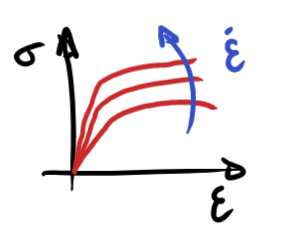
\includegraphics[width=\textwidth]{figures/burgers_cnst_strain_rate}
            \caption{}
            \label{subfig:burgers_cnst_strain_rate}
    \end{subfigure} \hfill
    \begin{subfigure}[b]{0.30\textwidth}
            \centering
            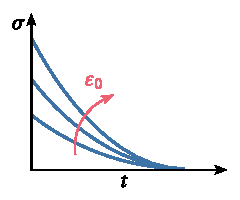
\includegraphics[width=\textwidth]{figures/burgers_stress_relax}
            \caption{}
            \label{subfig:burgers_stress_relax}
    \end{subfigure}
    \hfill
    \begin{subfigure}[b]{0.30\textwidth}
      \centering
      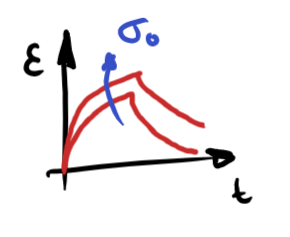
\includegraphics[width=\textwidth]{figures/burgers_creep_plus_recov}
      \caption{}
      \label{subfig:burgers_creep_plus_recov}
    \end{subfigure}
  \caption{Schematic response of the Burgers material in \subref{subfig:burgers_cnst_strain_rate} constant strain rate experiment, \subref{subfig:burgers_stress_relax} a stress relaxation experiment and a \subref{subfig:burgers_creep_plus_recov} creep experiment with recovery.}
\label{fig:burgers_mat_res}
\end{figure}

% \begin{remark}[Choice of internal variables]
%   A state variable is one of the set of variables that are used to describe the mathematical "state" of a dynamical system. Intuitively, the state of a system describes enough about the system to determine its future behaviour in the absence of any external forces affecting the system.
%   In general, they can be identified with the rheological elements able to storage energy, i.e., with the springs.
%   To see may the strain in the viscous element, may not be an appropriate choice consider, in the case of the Burgers material (see Equation~\eqref{}), a relaxation experiment where the strain is unknown and the external force is the strain rate which is zero.
%   Knowing the strain on the springs the the stress can be easily found and from these the evolution of the elastic strain from the flow rule.
%   If it was the viscous strains knwon not much could be done.
%   \colorbox{BurntOrange}{Include also stuff about structure.}
% \end{remark}

\paragraph{Linearity}
It is worth noting that infinitesimal thermoviscoelasticity is linear, in the sense that the response to the sum of two inputs is the sum of the responses to each of the inputs (see Figure~\ref{fig:linearity}).
In the context of viscoelasticity, this principle is called the Boltzmann-Volterra superposition principle \citep{wardIntroductionMechanicalProperties2004}.
Thus in the one-dimensional case, for discrete increases in strain $\Delta \varepsilon_i$ at instants $\tau_i$, $i=1,2,3,\dots$, the stress is given by
\begin{equation}
	\sigma (t) = \Delta \varepsilon_1 G(t - \tau_1) + \Delta \varepsilon_2 G(t - \tau_2) + \Delta \varepsilon_3 G(t - \tau_3) + \cdots
\end{equation}
If the increases in strain considered are rendered infinitesimal, the constitutive law found for the stress is the convolution integral in Equation~\eqref{eq:stress_constitutive_infinitesimal_viscoelasticity}.
This is entimately connected to the fact that the rate equations for the state variables are ordinary differential equations (see Equation~\eqref{eq:state_var_desc_burgers} for the Burgers material) and that as a material property, the relaxation modulus is only a function of time and not of strain, strain rate or stress (see Equation~\eqref{eq:relaxation_modulus_burgers} for the Burgers material).
The consequences of this linear behavior for the response of the material in relevant mechanical experiments are discussed shortly.
\begin{figure}[hbtp]
\centering
\begin{subfigure}[b]{0.49\textwidth}
            \centering
            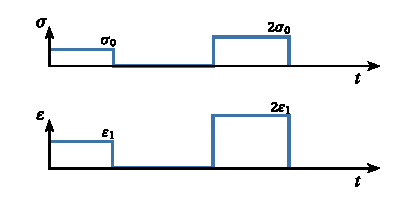
\includegraphics[width=\textwidth]{figures/elastic_linearity}
            \caption{}
            \label{subfig:elastic_linearity}
    \end{subfigure} \hfill
    \begin{subfigure}[b]{0.49\textwidth}
            \centering
            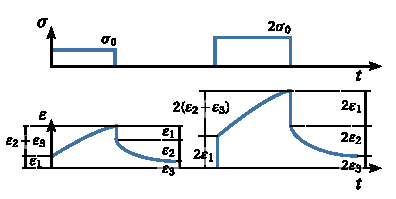
\includegraphics[width=\textwidth]{figures/viscoelastic_linearity}
            \caption{}
            \label{subfig:viscoelastic_linearity}
    \end{subfigure}
  \caption{Stress driven linear response of \subref{subfig:elastic_linearity} an elastic, and \subref{subfig:viscoelastic_linearity} a viscoelastic material. Adapted from \cite{wardIntroductionMechanicalProperties2004}.}
\label{fig:linearity}
\end{figure}

\paragraph{Limitations of infinitesimal viscoelasticity}
Infinitesimal viscoelasticity has however some major limitations, first among them the use of infinitesimal strains in the constitutive description of the material.
Semi-crystalline polymers, such as HDPE, can frequently achieve true strains in axial tests that exceed 1.5, far surpassing what could be considered small deformations \citep{gsellYieldTransientEffects1981}.

Furthermore, the Boltzmann superposition principle is frequently violated, and there is energy exchange between the different relaxation modes, implying that the relaxation modulus depends on strain, strain rate, and/or stress.
Semi-crystalline polymers exhibit nonlinear behavior that can be detected in a variety of mechanical experiments.
References to experimental results depicting this behavior can be found in Section~\ref{sec:relax_creep_dma}.
A comparison between a linear response and possible non-linear responses to the most common mechanical experiments is provided in what follows to understand the deficits of infinitesimal viscoelasticity.

Firstly, consider constant strain rate experiments ran at different strain rates.
At some point (see Equation~\eqref{eq:relax_mod_decomp}), a steady state will be reached, meaning $\dot {\bm\alpha} = 0,$ and the corresponding response in an infinitesimal viscoelastic model is either constant (liquid) or linear (solid) in the strain.
At any rate, for a given strain, the stress varies linearly with the strain rate and is proportional to the relaxation time, corresponding to so-called Newtonian viscosity \citep{matsuokaThermodynamicTheoryViscoelasticity1996} (see Figure~\ref{subfig:constant_strain_rate_expected}).
Neither of these two facts is always observed in practice.
For example, HDPE displays a marked strain hardening, as shown in the experimental results of \cite{gsellYieldTransientEffects1981}, e.g., which is not linear in the strain, i.e., the stiffness varies with the strain (see Figure~\ref{subfig:constant_strain_rate_nonlinear}).
Also, the stress corresponding to the steady state as a function of the strain rate often follows a power law (see e.g.,  \cite{gsellDeterminationPlasticBehaviour1979}) coinciding with so-called non-Newtonian viscosity (see Figure~\ref{subfig:constant_strain_rate_expected}).
Besides this, Matsuoka \citep{matsuokaThermodynamicTheoryViscoelasticity1996} emphasizes that the steady state stress grows unbounded with the strain rate according to infinitesimal viscoelasticity, which makes no physical sense.
Also, some semi-crystalline polymers exhibit more or less abrupt changes in flow behavior at a given stress, which is akin to plastic yield in rate-independent plasticity \citep{bergstromMechanicsSolidPolymers2015}.
\begin{figure}[hbtp]
\centering
  \begin{subfigure}[b]{0.49\textwidth}
            \centering
            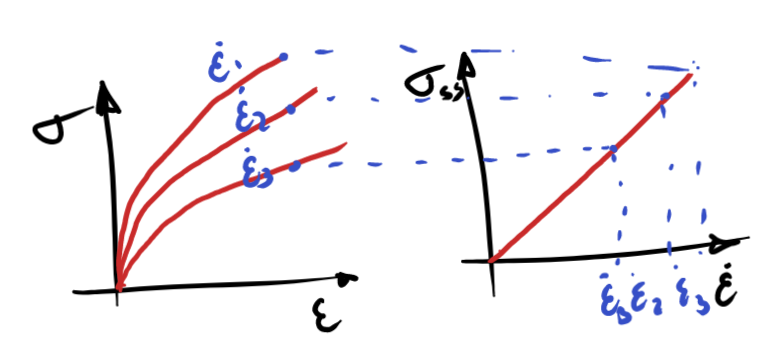
\includegraphics[width=\textwidth]{figures/constant_strain_rate_expected}
            \caption{}
            \label{subfig:constant_strain_rate_expected}
    \end{subfigure} \hfill
    \begin{subfigure}[b]{0.49\textwidth}
            \centering
            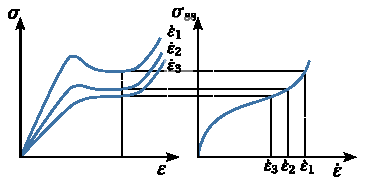
\includegraphics[width=\textwidth]{figures/constant_strain_rate_nonlinear}
            \caption{}
            \label{subfig:constant_strain_rate_nonlinear}
    \end{subfigure}
  \caption{Stress-strain curve and steady state stress-strain rate curve for a \subref{subfig:constant_strain_rate_expected} an infinitesimal viscoelastic material (linear) and a \subref{subfig:constant_strain_rate_nonlinear} nonlinear material.}
\label{fig:constant_strain_rate_results}
\end{figure}

Another nonlinear feature observed in semi-crystalline polymers is the dependence of the relaxation modulus and creep compliance on the strain and stress, in addition to time.
The expected linear behavior in a stress relaxation experiment is to obtain the same stress response up to a multiplicative constant, which is the initial strain.
Likewise, in a creep experiment the strain response divided by the stress is equal for experiments at different stress levels.
% See Figure~\ref{fig:relax_creep_expected} for a depiction of the expected linear and possible nonlinear behaviors.
The recovery may also display nonlinear features, that is, the strain recovered $\varepsilon_r$ will also depend on the initial strain $\varepsilon_0$ and how long the sample was strained, $t_0$, yielding completly different $\varepsilon/\varepsilon_0$ versus $\log t/t_0$ curves \citep{ferryViscoelasticPropertiesPolymers1980}.
% \begin{figure}
%   \includegraphics[width=0.9\textwidth]{example-image-a}
%   \caption{Expected behavior of a infinitesimal viscoelastic material and nonlinear alternatives in a) stress relaxation experiment, b) in a creep experiment. }
% \label{fig:relax_creep_expected}
% \end{figure}


\section{Finite linear viscoelasticity}
The infinitesimal viscoelatic model can be derived assuming that the stress depends only on the "magnitude" of the deformation history to the first order (see \cite{colemanFoundationsLinearViscoelasticity1961} or \cite{christensen2013theory}).
This is automatically satisfied if only small strains are considered.
However, Coleman and Noll \citep{colemanFoundationsLinearViscoelasticity1961} point out that finite deformations can also be considered, as long as the motion is slow enough when compared with the material's rate of "forgeting".
The stress strain constitutive relation is still described as a convolution integral (see Equation~\eqref{eq:stress_constitutive_infinitesimal_viscoelasticity}), and may be frequently described by ordinary differential equations, where instead of the infinitesimal strain tensor, a strain measure compatible with finite strains, e.g., the Green-Lagrange strain tensor, can be employed.
This approach to viscoelasticity allows for finite strains, however it is still linear with respect to the strain measure,--not the displacement, since the former are nonlinear functions of the latter--, thus, respecting the Boltzman superposition principle and keeping the relaxation spectrum depending only on time.
As such, this model won't display most of the required nonlinear effects observed in semi-crystalline polymers and described in the previous chapter.
In addition, since the dissipation is a second order effect, the state of the material remains close to thermodynamical equilibrium, so that the dissipation will not contribute as a source in the heat conduction equation (Equation~\eqref{eq:heat_conduction}).

\section{Single integral models}
Another set of approaches that seeks to generalize the results of infinitesimal viscoelasticity is based on the integral constitutive equation for the stress as a function of the strain in Equation~\eqref{eq:stress_constitutive_infinitesimal_viscoelasticity}.
These models include nonlinear phenomena while considereing only small strains \citep{wardIntroductionMechanicalProperties2004}.
For example, the model of Pipkin and Rogers is given by \citep{wardIntroductionMechanicalProperties2004}
\begin{equation}
	\sigma(t) = \int_{-\infty}^t R(t-\tau, \varepsilon(\tau))\frac{\partial \varepsilon}{\partial \tau}\ d\tau,
\end{equation}
where $R$ is a nonlinear stress relaxation modulus depending on both time and strain, incorporating nonlinear effects into the material's infinitesimal viscoelastic constitutive description.

A list of models of this type, including the models of Leaderman, Pipkin and Rogers, Schapery, and Bernstein, Kearsley and Zapas (BKZ) can be found in \cite{wardIntroductionMechanicalProperties2004} and \cite{malkinRheologyConceptsMethods2017}.
According to Ward and Sweeney \citep{wardIntroductionMechanicalProperties2004}, Smart and Williams \citep{smartComparisonSingleintegralNonlinear1972} assessed the three models' performance when applied to tensile stretching of polypropylene and poly(vinyl chloride) fibers, but only up to modest strains (4\%).
At these strains, the BKZ model proved to be of limited interest, while the Pipkin and Rogers model, albeit being simpler than Schapery's theory, yielded a somewhat inferior result.
Moreover, Turner \citep{turnerStrainResponsePlastics1966} concludes about single integral models that viscoelastic behavior in general cannot be discussed simply in terms of a stress-strain-time relationship and a modified superposition integral.

With particular relevance to the modeling of semi-crystalline polymers, Popelar \citep{popelarViscoelasticMaterialCharacterization1990} modeled MDPE and HDPE employing Schapery's nonlinear viscoelasticity with good results.
The experimtal test used for validation included constant strain rate uniaxial traction tests with strain rates ranging from \SIrange{1e-5}{1e-1}{\per\second} and temperatures from \SIrange{23}{77}{\celsius} and a maximum strain of 0.25.
Regarding the free energies corresponding to these stress-strain constitutive relationhips, Gurtin and Hrusa \citep{gurtinEnergiesNonlinearViscoelastic1988} present a discussion on the topic.
This class of models will not be discussed further in the text since, due to their formulation in terms of convolution integrals, they are not particularly appropriate for application in computational mechanics.

\section{Descriptions based on rheological models wiht nonlinear elements}

A viscoelastic constitutive model fit for large strains and capable of capturing the required nonlinear behaviors can often be achieved by specifying nonlinear laws for the behavior of the viscous and elastic elements in a rheological model.
It is by far the most common approach, and to introduce it, the laws available for viscous elements are presented first, followed by the corresponding laws for elastic elements.
The kinematic decomposition required to generate a large strain three-dimensional model, as well as the changes required for the introduction of the thermal field, are discussed.
Finally, the most relevant models from the literature that follow this approach are presented.

% \begin{remark}[Phenomenological vs. First principles]
% 	A phenomenological model rests on fitting parameters and empirical assumptions.
% 	A first principle rests on reasoning from first principles.
% 	What are first principles? It depends on the chosen abstraction level.
% 	We have continuum mechanics, kinetic theory/statistical mechanics, molecular dynamics and quantum mechanics.
% 	Here only continuum mechanics and kinetic theroy are considered.
% 	Give examples? What moves from one to the other? \colorbox{BrickRed}{Complete this!!!!}
% \end{remark}

\subsection{Viscous elements}
\label{sec:viscous_elements}

Plastic flow is a kinetic process, as pointed out by Frost and Ashby \citep{frostDeformationmechanismMapsPlasticity1982}, therefore, the strength of a solid depends on both strain and strain-rate, in addition to the temperature.
This runs counter to the useful concept of a yield strength, below which there is no flow and above which flow is fast.
According to the same authors, this would only be strictly true at absolute zero.
The corresponding theoretical flow stress is often called the mechanical threshold or athermal strength.
Furthermore, flow below that mechanical threshold is due to thermally activated kinetic processes, i.e., their rate depends on the thermal fluctuations of the kinetic units.
For the sake of completeness, it should be mentioned that there are kinetic processes that become relevant when the loading exceeds the mechanical threshold, coinciding with very high strain rates, and which do not necessitate thermal activation to occur \citep{kocks1975thermodynamics}\footnote{In the context of polycrystalline materials, where slip is the main deformation mechanism the former correspond to so-called jerky glide and the latter to continuous glide \citep{kocks1975thermodynamics}.}.
These are beyond the scope of the present work.

To better understand how thermal fluctuations allow for flow, consider that at a given temperature in a solid, the kinetic units perform thermally driven oscillations of random magnitude near an equilibrium position.
If the motion of the kinetic units coincides with their permanence near that equilibrium state the behavior of the solid will be elastic.
On the other hand, flow happens when the energetic barrier $\Delta H$ bounding the equilibrium state is cleared.
This is the energy of activation at \SI{0}{\kelvin} when no force is acting on the material \citep{kocks1975thermodynamics}.
Employing the Boltzmann distribution from statistical mechanics to calculate the probability of a thermal fluctuation providing enough energy to overcome the energy barrier, the rate of transition between states is given in the form of the Arrhenius equation, written in this context as
\begin{equation}
	k = A\exp\left(-\frac{\Delta H}{k_BT}\right),
\end{equation}
where $k_B$ is Boltzmann's constant, $A$ is the pre-exponential factor, $\varepsilon_0$ is the height of the energy barrier.
The pre-exponential term can be interpreted as the rate of attempts to move over the transition state \citep{atkins2010atkins}.
According to Kocks et al. \citep{kocks1975thermodynamics}, it is related to one of two extreme frequencies: either the "atomic" frequency, i.e., the frequency of uncorrelated atomic motions, or the kinetic unit ground frequency, correlated with the overcoming of many of obstacles at the same time.
The inverse of the this rate, i.e.,
\begin{equation}
	\theta = \frac{1}{A}\exp\left(\frac{\Delta H}{k_B T}\right),
\end{equation}
is the relaxation time of the process.

To consider the effect of applying a stress to the material, take into account that the work provided by that stress will be discounted from the total energy required to overcome the kinetic unit's obstacle to motion.
The free Gibbs energy, also known as free enthalpy, is that missing portion of energy that must be supplied by a thermal oscillation.
Without factoring in the thermal fluctuations, the motion would occur only if the work supplied by the stress was larger than the energy barrier.
Moreover, if the free energy of the kinetic unit is greater after crossing the barrier, some of the plastic work was not dissipated, some energy remaining latent in the material.
On the other hand, the free enthalpy of the kinetic unit is always lower after crossing the barier; otherwise, there would be no greater probability of crossing in one direction than the other (see Figure~\ref{fig:site_model_theory}).
For more details see \cite{kocks1975thermodynamics}.
\begin{figure}
	\centering
	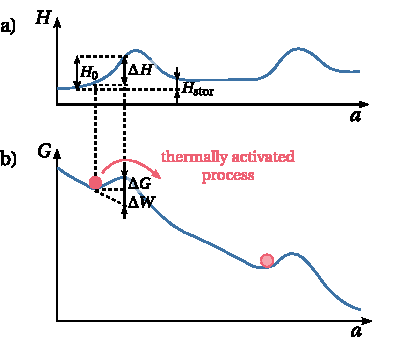
\includegraphics{figures/site_model_theory}
	\caption{Transition of a kinetic unit between two states. a) Free energy. b) Free enthalpy.}
\label{fig:site_model_theory}
\end{figure}

Thus, following the procedure outlined by Eyring \citep{eyringViscosityPlasticityDiffusion1936}, the shearing force acting on the system and its effect on the flow of the kinetic units can be considered.
Its presence will lead to a different rate of jumps in the forward and backward directions, which in energetic terms means lowering the energy of the final state and increasing the energy of the initial state.
Assuming similar activation volumes, and subtracting the rate of kinetic units moving against the shearing force from those moving along with the shearing force, $\tau$, the strain rate obtained is
\begin{equation}
	\label{eq:eyring_model}
	\dot \gamma = \dot\gamma_0 \exp\left(-\frac{\Delta H}{k_BT}\right)\sinh\left(\frac{v\tau}{k_BT}\right),
\end{equation}
where $v$ is the so-called activation volume, and it can be identified with the product of the area swept out by the mobile unit in moving from one local free energy minimum to the next and the resolved component in the direction of the applied stress of the distance moved by the kinetic unit.

According to the same author, for ordinary flow, $v\tau$ is much smaller than $k_B T$, thus, the expression for Newtonian viscous flow is recovered as
\begin{equation}
  \label{eq:newton_fluid_flow_rule_scalar}
	\dot \gamma = \frac{\dot \gamma_0 v}{k_B T}\exp\left(-\frac{\Delta H}{k_BT}\right)\tau=\frac{1}{\eta}\tau,
\end{equation}
where $\eta$ is the viscosity.
On the other hand, for plastic flow, when $\tau$ is large, the flow rule comes out to be
\begin{equation}
\label{eq:flow_rule_thermally_activated}
	\dot\gamma = \dot \gamma_0 \exp\left(-\frac{\Delta H - v \tau}{k_B T}\right)=\dot \gamma_0 \exp\left(-\frac{\Delta G(\tau)}{k_B T}\right),
\end{equation}
which coincides with a negligible rate in the backwards direction.
The contribution of hydrostatic pressure can also be accounted for in this framework in a similar way to the shearing force, i.e.,
\begin{equation}
  \label{eq:eyring_w_pressure}
	\dot\gamma = \dot\gamma_0 \exp\left(-\frac{\Delta H - v \tau + \Omega p}{k_B T}\right),
\end{equation}
where $\Omega$ is the activation volume corresponding to the hydrostatic pressure.
This can be justified in terms of experimental results, where the stress response of polymers shows a pressure dependence, in part due to the low bulk moduli of polymers (~\SI{5}{\giga\pascal}, compared with metals ~\SI{100}{\giga\pascal}) \citep{wardIntroductionMechanicalProperties2004}.
A suitable expression for the effective stress on the kinetic units is found to be a linear combination of shear stress and hydrostatic pressure, similar to the Mohr-Coloumb yield criterion.
From the expressions, it is clear that higher shear stresses lead to higher flow rates, with the hydrostatic pressure having the reverse effect.

According to Fotheringham and Cherry \citep{fotheringhamRoleRecoveryForces1978} it is not clear that the activation volumes in the forward and backward direction are the same.
However, note that when the expression is employed to describe plasticity this is not relevant, as only one activation volume has to be considered.
In fact, more general rate equations for thermal activated flow can be found in \cite{brinkmanMechanicalThermodynamicalTheory1957} or \cite{kocks1975thermodynamics}.

The experimental determination of the parameters in these models are discussed, e.g., in \cite{evansThermallyActivatedDeformation1969}, \cite{conradAthermalComponentFlow1970} and \cite{kocks1975thermodynamics}, through the use of differential tests, changes of strain-rate in a constant strain-rate test, or stress level steps in a creep experiment.

% \colorbox{BrickRed}{Zhurkov \citep{s.n.zhurkovKineticConceptStrength1965} found good results employing the Eyring model to predict the time to failure for uniaxial tensile specimens of some 50 materials, measured in some cases over ten decades of time, has suggested a universal rate relation between lifetime, stress, and temperature of said form.
% The constant 'r 0 is essentially the reciprocal of the natural oscillation frequency of atoms in the solid, Uo is the binding energy on the atomic scale, and y is proportional to the disorientation of the molccular structure.
% Assuming the kinetic nature of bond destruction through the thermofluctuation mechanism, dircct experimental verification of the phenomenon for polymers has been obtained using electron paramagnetic resonance.}

Roberston \citep{robertsonTheoryPlasticityGlassy1966} presents an alternative to the Eyring model applicable to glassy polymers.
The author considers a molecular model in which the shear-stress field is introduced as a bias on the rotational conformation of backbone bonds.
The temperature at which the maximum fraction of flexed bonds is observed is estimated, and pluged into the WLF equation to compute the corresponding viscosity, and hence the equation for the strain rate.
Comparisons with results for PS and PMMA are provided.
Duckett et al. \citep{duckettStrainrateTemperaturePressure1970} also employ this models to fit the responses of PMMA and PET.

El-Qoubaa and Othman \citep{el-qoubaaStrainRateSensitivity2016} provide an implicit flow rule, while seeking to model the yield stress of PEEK as a function of the strain rate and the temperature.
The equation proposed is
\begin{equation}
	\label{eq:elquobaa_ree_eyring_stress}
	\tau = \frac{k_B T}{v(\dot \gamma, T)}\ln\left(\frac{\dot\gamma}{\dot\gamma_0}\right),
\end{equation}
where the activation volume, $v$, on the strain rate and the temperature according to
\begin{gather}
	v(\dot\gamma, T) = v_0(T)\exp\left(-\sqrt{\frac{\dot\gamma}{\dot \gamma_c(T)} }\right),\\
	v_0(T) = v_1 + v_2 \left(\frac{T}{T_g}\right)^n,\\
	\dot \gamma_c (T) = \dot \gamma_1 \exp(q T),
\end{gather}
$T_g$ is the glass transition temperature, and $\tau_1$, $m$, $r$, $v_0$, $v_1$, $n$, $\dot\gamma_1$ and $q$ are material constants.
The authors find a good agreement between the model and experimental data.
An implicit law for the strain rate $\dot \gamma$ can be written using Equation~\eqref{eq:elquobaa_ree_eyring_stress}.

The models described so-far are often termed velocity-controlled, as they assume that yield (see Remark~\ref{rmrk:yield_polymer}) will occur when the strain rate of the viscous element, identified with the movement of kinetic units, is equal to the impressed rate of deformation \citep{fotheringhamRoleRecoveryForces1978}.
These models can also be thought of as specifying that the presence of stress causes an increase in pre-existing flow processes in the material, such that the stress corresponding to their flow equals the loading stress \citep{wardIntroductionMechanicalProperties2004}.

Notice that despite mentioning the existence of deformation mechanisms corresponding to the motion of kinetic units, the models presented in the previous paragraphs do not attempt to model the specific physical events directly.
Alternatively, in the case of nucleation-controlled models for polymer plastic flow, the free enthalpy is directly modeled to determine the energy required in the nucleattion and motion of the kinetic units \citep{fotheringhamRoleRecoveryForces1978, wardIntroductionMechanicalProperties2004}.

Argon \citep{argonTheoryLowtemperaturePlastic1973} proposes a model for plastic deformation of glassy polymers where the deformation mechanism is the buckling of the polymer chains via the action of a pair of opposed kinks.
The expression found for the free enthalpy is
\begin{equation}
	\label{eq:argon_model_free_enthalpy}
	\Delta G(\tau)=\frac{3 \pi \mu \omega^2 a^3}{16(1-\nu)}\left[1-\left(\frac{\tau}{\hat \tau}\right)^{5 / 6}\right],
\end{equation}
where $\mu$ and $\nu$ are the shear modulus and Poisson coefficient, $\hat \tau$ is the athermal strength defined as
\begin{equation}
  \label{eq:athermal_strength_elasticity_rel}
	\hat \tau = \frac{0.077 \mu}{1-\nu},
\end{equation}
$\omega$ the net angle of rotation of the molecular segment between the initial configuration and the activated configuration, and $a$ the mean molecular radius.
The relationship between the athermal strength and the shear modulus in Equation~\eqref{eq:athermal_strength_elasticity_rel} can be used to establish the temperature of the athermal dependence \citep{haoUnifiedAmorphousCrystalline2022}.

In the case of amorphous polymers, however, Ward and Sweeney \citep{wardIntroductionMechanicalProperties2004} mention that computer simulations of polymer chains at the atomic level on both glassy atactic polypropylene and polycarbonate did not yield a dominant deformation mechanism that should be the target of modeling.

In the case of semi-crystalline polymers, the picture changes in the sense that, as reviewed in the previous chapter (Chapter~\ref{ch:thermomechanical_behavior_semi_crystalline_polymer}), the plastic behavior of the material is tightly linked to deformation mechanisms in the crystalline phase.
There is extensive modeling of plastic behavior in polycrystalline solids with direct identification of the kinetic units as dislocations in the crystal\footnote{A dislocation loop can be defined as the demarcation line, in one slip plane, between an area that has splipped and a surrounding area that has not.}.
Their motion can be modeled, according to Kocks et al. \citep{kocks1975thermodynamics}, as in Equation~\eqref{eq:flow_rule_thermally_activated} where
\begin{equation}
	\label{eq:pre_exponential_def}
	\dot \gamma_0 = b\rho_m L \nu_G,
\end{equation}
where $b$ is the Burgers vector\footnote{The Burgers vector is a vector that represents the magnitude and direction of the lattice distortion resulting from a dislocation in a crystal lattice.} with dimensions of length, $\rho_m$ is the mobile dislocation densitiy with dimensions of dislocation length per volume, $L$ the mean path of a mobile dislocation between inception and arrest at an obstacle and $\nu_G$ the frequency factor associtated with the attempt rate of the nucleation process.
At still moderate stresses the average velocity is mainly controlled by thermally activated processes where the dislocations wait until a thermal fluctuation allows them to clear the obstacle.

Argon \citep{argonPhysicsDeformationFracture2013a} presents the three relevant modes of dislocation nucleation in polymer lamellae as the nucleation of a monolithic straight screw-dislocation line from the edge of a lamella (mode A), nucleation of a screw-dislocation half loop from the narrow edge of a lamella (mode B), and nucleation of an edge-dislocation half loop from the wide face of a lamella (mode C).
The respective free enthalpies for each mode are
\begin{align}
	\Delta G_A(\tau)&=\frac{\mu b^2}{4 \pi} \ln\left(\frac{\tau_c}{\tau}\right),\\
	\Delta G_B(\tau)&=\frac{\mu b^2}{4 \pi} \frac{1-(\tau/\tau_c)^{2 / 3}}{(\tau/\tau_c)^{1.25} },\\
	\Delta G_C(\tau)&=\frac{\mu b^3}{1-v} \frac{1-(\tau/\tau_c)^{1 / 3}}{(\tau/\tau_c)^{1.15} },
\end{align}
where $\tau_c$ is the ideal shear force.
Expressions for the mobile dislocation density are also presented by the same author as
\begin{equation}
	\rho_m = \frac{\chi p N \lambda}{\lambda \Lambda^2},
\end{equation}
where $\lambda$ is the length of the dislocation produced, $p$ the probability of a successful nucleation event at a site, $\chi$ is the level of crystallinity and $N = 2\Lambda/h$ is the number of possible nucleation sites in the representative volume $\lambda \Lambda^2$ allocated to a lamella, and $h$ is the interplanar spacing.
The mobile discolation densitiy, $\rho_m$, or the ideal shear force, $\tau_c$, can also be taken as an internal variable and made to evolve according to a rate equation.
See \cite{klahn1970strain} and \cite{kocks1975thermodynamics} for thorough discussions on the modeling of the deformation mechanisms in crystalline solids.

For an amorphous or semi-crystaline polymer,  Equations~\eqref{eq:flow_rule_thermally_activated} and \eqref{eq:pre_exponential_def} can still be employed, with a slightly different interpretation for the quantities involved and keeping in mind that the kinetic units are not as precisely defined as the in case of crystalline solids.
Thus, the strain rate is still given by
\begin{equation}
  \label{eq:plaston_formula}
  \dot \gamma = b \rho_m \bar{v}_m,
\end{equation}
i.e., by the product of the density of kinetic units responsible for the deformation, $\rho_m$, the amount of displacement per kinetic unit, $b$, and their average velocity, $\bar v_m$.
This velocity is approximately given by
\begin{equation}
  \bar v_m = L \nu_G \exp\left(-\frac{\Delta G(\tau)}{k_B T}\right),
\end{equation}
where $L$ is the mean free path of the kinetic unit, $\nu_G$ is the rate of attempts to move over the obstacle impeding its motion, and the Arrhenius term is the probability that the thermal fluctuations will supply the energy necessary to overcome said obstacle \citep{gsellYieldTransientEffects1981, gilmanPLASTICWAVEMYTH1992}.

Finally, one must keep in mind that both the nucleation and velocity controlled models produce similar expressions, but their interpretations differ \citep{fotheringhamRoleRecoveryForces1978}.

The deformation mechanism discussed so far concerned the motion of kinetic units by themselves.
However, some kinetic processes are cooperative in nature, occurring only when several kinetic units act in unison.
In fact, Cherry and Holmes \citep{cherryYieldAdhesiveJoints1969} mention that the fited values to the activation volume in Eyring's model are to large to agree with their corresponding physical interpretation (see Equation~\eqref{eq:eyring_model}.)
To model this situation, Fotheringham and Cherry \citep{fotheringhamCommentCompressionYield1976, fotheringhamRoleRecoveryForces1978} assume that $n$ kinetic units all following the Eyring model are needed to substantiate a deformation mechanism.
The expression found for the flow rate is
\begin{equation}
  \label{eq:cooperative_flow_rule}
	\dot{\gamma}=\dot \gamma_0 \sinh ^n\left(\frac{v \tau}{2 k T}\right) \exp \left(-\frac{n \Delta H}{k T}\right),
\end{equation}
where the notation employed retains its meaning from previous paragraphs and a temperature below the glass transition temperature is assumed.
Richeton et al. \citep{richetonFormulationCooperativeModel2005} look to model the yield stress of amorphous polymers, extending the cooperative model to temperatures above the glass transition temperature.
They achieve this proposing
\begin{equation}
		\dot{\gamma}=\dot \gamma_0 \exp\left(\frac{\ln 10\cdot c_1^g(T - T_g)}{c_2^g + T - T_g}\right) \sinh ^n\left(\frac{v \tau}{2 k T}\right) \exp \left(-\frac{\Delta H}{k T_g}\right),
\end{equation}
for temperatures above $T_g$, where $c_1^g$ and $c_2^g$ are the WLF parameters \citep{wardIntroductionMechanicalProperties2004}.
Some of the same authors \citep{richetonThermodynamicInvestigationYieldstress2007} compare the models of Eyring (see Equation~\eqref{eq:eyring_model}), Argon (see Equation~\eqref{eq:argon_model_free_enthalpy}) and their cooperative model in the prediction of PMMA's and PC's yield stress.

Other models, however, do not fit neatly into the scheme outlined above.
% \colorbox{BrickRed}{See \cite{kellyInfluenceLimitingDislocation1974} and gen with $n$ for the exponential law.}
Power laws are fairly common empirical laws for the flow rule \citep{brownPowerlawCreepEquation1980}.
They are given, for example, as \citep{bergstromMechanicsSolidPolymers2015}
\begin{equation}
	\label{eq:flow_rule_power_law}
	\dot \gamma = \dot \gamma_0 \left(\frac{\tau}{\hat \tau}\right)^m,
\end{equation}
where $m$ is a material parameter and $\hat \tau$ a reference stress.
Perzyna \citep{perzynaConstitutiveEquationsRate1963}, e.g., proposes
\begin{equation}
\label{eq:flow_rule_perzyna}
  \dot \gamma = \frac{1}{\mu}\left(\frac{\langle\tau - \hat\tau\rangle}{\hat\tau}\right)^{1/\varepsilon},
\end{equation}
to describe the rate sensitivity of plastic materials.
$\langle\bullet\rangle$ denotes the ramp function, defined as $\langle x\rangle = (|x| + x) /2$, and $\mu$ and $\epsilon$ are material paramters.
Another law available for the strain rate is \citep{kellyInfluenceLimitingDislocation1974, bodnerLargeDeformationElasticViscoplastic1972}
\begin{equation}
  \label{eq:exp_flow_law}
	\dot \gamma = \dot \gamma_0 \exp\left(-\left(\frac{\hat \tau}{\tau}\right)^n\right),
\end{equation}
where $n$ is a material parameter.
According to Bodner and Partom \citep{bodnerLargeDeformationElasticViscoplastic1972}, they are suggested by both direct measurements and theoretical consideriations of the average velocity of mobile discolations as a function of the applied stress (see Equation~\eqref{eq:pre_exponential_def}).

Yet another model available in the literature, based on reptation \citep{doiDynamicsConcentratedPolymer1978a}, is described by Bergström and Boyce \citep{bergstromConstitutiveModelingLarge1998, bergstromConstitutiveModelingTimedependent2001}.
The flow is due in part to the Brownian motion of the polymer chains, in addition to thermally activated events, yielding the following flow rule
\begin{equation}
	\label{eq:bb_reptation_model}
	\dot \gamma = C_1(\lambda_\text{chain} -1 + \xi)^{C_2}\left(\frac{\tau}{\hat\tau}\right)^{m},
\end{equation}
where $\lambda_\text{chain}$ is the chain stretch and $C_1$, $C_2$, $m$ and $\hat \tau$ are material parameters.
The constant $\xi\approx 0.01$ is introduced to eliminate the the singularity at $\lambda_\text{chain}=1$.

According to de Souza Neto et al. \citep{desouzanetoComputationalMethodsPlasticity2008}, more flow rules can be generated by multiplying several simpler laws, including those already provided.
For example, assuming that $\dot \gamma$ is a function of the stress, time and temperature, one can write
\begin{equation}
	\dot \gamma = \dot \gamma(\tau, t, T) = f_\sigma (\tau) f_t(t) f_T(T),
\end{equation}
where $f_\tau$, $f_t$ and $f_T$ are possibly experimentally defined functions.

% Table~\ref{tab:flow_rules} summarizes the different flow rules discussed so far.
% It includes the application domain of each and some authors who have used them in the context of polymer modeling.
% \begin{landscape}
% \begin{table}[!ht]
% \caption{Summary of the flow rules employed in the modeling of polymers.}
% \label{tab:flow_rules}
%   \begin{tabular}{lcccl}
%   \hline
%   Model\vphantom{\Big\vert} & Equation  & Domain of application & Observations \\ \hline\hline
%   Newton viscosity & $\displaystyle	\dot \gamma = \frac{\dot \gamma_0 v}{k_B T}\exp\left(-\frac{\Delta H}{k_BT}\right)\tau=\frac{1}{\eta}\tau,$  (Eq.~\eqref{eq:newton_fluid_flow_rule_scalar}) & $v\tau \ll k_B T$  & Describes ordinary flow.  \\
%   Eyring's model & $\displaystyle\dot \gamma = \dot\gamma_0 \exp\left(-\frac{\Delta H}{k_BT}\right)\sinh\left(\frac{v\tau}{k_BT}\right)$ (Eq.~\eqref{eq:eyring_model}) & $\tau < \Delta H/v$   &  \\
%   Argon's model &  &   & \\
%   Cooperative model &  &  &    \\
%   Richeton's model & & &  \\
%   \hline\hline
%  \end{tabular}
% \end{table}
% \end{landscape}

\paragraph{Structure variables}
So far all the constitutive descriptions provided for the strain rate neglect to consider the material's thermomechanical history.
As already discussed in Section~\ref{sec:constitutive_modeling}, a set of appropriate internal variables, in this context also called structure variables (see \cite{kocks1975thermodynamics} and \cite{frostDeformationmechanismMapsPlasticity1982}), is employed to capture the contribution of said history to the thermomechanical response of the material.
Thus, the implicit assumption so far is either that the structure remains constant during flow, i.e.,
\begin{equation}
  \bm \alpha = \bm \alpha_0,
\end{equation}
or that it has reached as a steady state, i.e.,
\begin{equation}
  \dot{\bm \alpha} = \bm 0.
\end{equation}

Either of these hypothesis is often unreasonable, and fails to explain the nonlinear behavior of polymers.
This shortcoming is especially visible in the ability to capture the shape of the transient in a constant strain rate test, be it the characteristic strain softening of many glassy polymers or the double yield of various semi-crystalline polymers.
The most common targets of modeling are the athermal strength, $\hat \tau$, and the mobile dislocation density, $\rho_m$, (see Equations~\eqref{eq:flow_rule_thermally_activated} and \eqref{eq:pre_exponential_def}).

Regarding the athermal strength $\hat \tau$, two natural assumptions are that it may depend on both the plastic strain $\gamma$ and time, thus, by the chain rule, one finds
\begin{equation}
  \dot{\hat \tau} = h \dot\gamma - r,
\end{equation}
where $h\equiv \partial \hat \tau/\partial \gamma |_t$ corresponds to a hardening rate and $r\equiv - \partial \hat \tau/\partial t|_\gamma$ denotes a recovery or, in the case of polymers, also aging rate.
Hardening is expected if there is an increase in the number of obstacles to the motion of the kinetic unit \citep{kocks1975thermodynamics, hasanConstitutiveModelNonlinear1995}.
The minus sign in the definition of the recovery/aging rate is introduced to enforce a decrease in the athermal strength connected to either recovery or aging.
That said, Boyce et al. \citep{boyceLargeInelasticDeformation1988} concludes that aging in PVC may increase its athermal strength.

Bodner and Partom \citep{bodnerConstitutiveEquationsElasticViscoplastic1975} propose
\begin{equation}
  \hat \tau = {\hat \tau}_1 + ({\hat \tau}_0 - {\hat \tau}_1)\exp\left(-\frac{m}{{\hat \tau}_0}w^p\right),
\end{equation}
where ${\hat \tau}_0$ and ${\hat \tau}_1$ are the initial and final athermal strengths, respectively, and $m$ a material property.
Comparing with the original text, a multiplicative factor $((n+1)/n)^{1/n}$ is neglected as it tends to 1 for large $n$.
The plastic work, $w^p$, is defined as $\int \tau\dot \gamma\ dt$, in the one-dimensional case.
The corresponding rate equation can be written as \citep{zairiElastoviscoplasticConstitutiveEquations2007}
\begin{equation}
  \label{eq:bodner_partom_rate_eq}
  \dot{\hat \tau} = m\left(\frac{{\hat \tau}_1 - {\hat \tau}}{{\hat \tau}_0}\right)\dot w^p.
\end{equation}

Zaïri et al. \citep{zairiElastoviscoplasticConstitutiveEquations2007} propose similar rate equations for partial contributions, $\hat \tau^{(1)}$ and $\hat \tau^{(2)}$, to the athermal strength, $\hat \tau$, when modeling glassy polymers.
The former concerns the hardening effect of the network aligniment, such that the corresponding rate equation is defined as
\begin{equation}
  \dot{\hat\tau}^{(1)} = m\left(\frac{\hat\tau^{(1)} - (1 - \alpha)\hat\tau^{(1)}_0}{\hat\tau^{(1)}_0}\right)\dot w^p,
\end{equation}
where $m$ is material parameter, $\hat\tau^{(1)}_0$ is the initial athermal strength and $\alpha$ a hardening parameter.
In turn, the latter accounts for the effect of strain softening, with the corresponding rate equation given as
\begin{equation}
  \dot{\hat\tau}^{(2)} = p\left(\frac{\hat\tau^{(2)}_1 - \hat\tau^{(2)}}{\hat\tau^{(2)}_1}\right)\dot w^p.
\end{equation}
where $p$ is a material parameter and $\hat\tau^{(2)}_1$ is a final partial athermal strength, such that
\begin{equation}
  \label{eq:rate_eq_zairi}
  \dot{\hat \tau} = \dot{\hat\tau}^{(1)} + \dot{\hat\tau}^{(2)}.
\end{equation}
The solution to both equations can be found substituting the appropriate values into Equation~\eqref{eq:bodner_partom_rate_eq}.

Note that, despite the use of the plastic work instead of the plastic strain in the definition of the rate equations just discussed, their use is often equivalent.
This is because the mapping between the two can be made one-to-one such that $\hat \tau(\gamma)=\tilde{\hat \tau}(w^p)\equiv \hat\tau(w^p(\gamma))$.
See \cite{desouzanetoComputationalMethodsPlasticity2008} for the full derivation.

Boyce et al. \cite{boyceLargeInelasticDeformation1988} propose an entirely similar rate equation for the athermal strength in a glassy polymer.
The corresponding strain softening is described as
\begin{equation}
  \label{eq:rate_equation_bpa}
	\dot{\hat \tau}=h \left(1-\frac{\hat \tau}{\hat \tau_{1} \left(T, \dot{\gamma}\right)}\right)\dot{\gamma}
\end{equation}
employing however the strain rate as the "driving force" behind its change.
The initial structure is represented by the value of $\hat \tau$ at the upper yield point, $\hat \tau_0$, $h$ is the slope of the yield drop with respect to the strain, $\hat \tau_1$ is the value $\hat \tau$ reaches at steady state, i.e., the "preferred" structure, and, as indicated, $\hat \tau_1$ may depend on temperature and strain rate.
This choice for the rate equation of the athermal strength enables the modeling of the distinctive glassy polymer strain softening.

In their attempt to model semi-crystalline polymers, Ahzi et al. \citep{ahziModelingDeformationBehavior2003} propose
\begin{equation}
  \label{eq:rate_equation_power}
  \dot{\hat \tau} =  \frac{\hat \tau}{n}\left(\frac{\hat\tau_0}{\hat\tau}\right)^n\dot \gamma,
\end{equation}
as the rate equation for the athermal strength $\hat\tau$, where $\hat\tau_0$ is the corresponding initial value and $n$ is a hardening coefficient.

Seeking to model the effect of manufacturing-induced voids in polymer-based composites, Chowdhury et al. \citep{chowdhuryEffectsManufacturingInducedVoids2008} present an extension of Equation~\eqref{eq:rate_equation_bpa}.
It describes the transition from a pre-defined initial yield stress, $\hat\tau_0$, to a peak yield stress, $\hat\tau_1$, followed by strain softening to a saturated state, $\hat\tau_2$.
The corresponding rate equation is
\begin{equation}
	\label{eq:two_athermal_strength_evo}
	\dot{\hat\tau}=H_1(\gamma)\left(1-\frac{\hat\tau}{\hat\tau_1}\right) \dot{\gamma}+H_2(\gamma)\left(1-\frac{\hat\tau}{\hat\tau_2}\right)\dot{\gamma},
\end{equation}
with the smooth Heaviside-like functions $H_i$, $i=1,2$ given by
\begin{equation}
	H_1(\gamma)=-h_1\left\{\tanh \left(\frac{\gamma-\gamma^p}{f \gamma^p}\right)-1\right\} ; \quad H_2(\gamma)=h_2\left\{\tanh \left(\frac{\gamma-\gamma^p}{f \gamma^p}\right)+1\right\},
\end{equation}
where $h_1$ and $h_2$ are the hardening (softening) parameters, $f$ the smoothing factor and $\gamma^p$ the plastic strain at the peak yielding point.
This approach is also pursued by Hao et al. \citep{haoUnifiedAmorphousCrystalline2022}, where however a fourth athermal shear stress $\hat \tau_3$ is considered, connected to the yield of the crystalline phase in a semi-crystalline polymer.
According to the authors, this property can depend on the temperature, the strain rate, the crystallinity and humidity.
The rate equation for the athermal strength $\hat\tau$ is given similarly to Equation~\eqref{eq:two_athermal_strength_evo} as
\begin{equation}
  \label{eq:rate_equation_hao}
	\dot{\hat\tau}=H_1(\gamma) \left(1-\frac{\hat\tau}{\hat\tau_1}\right)  \dot{\gamma}+H_2(\gamma) \left(1-\frac{\hat\tau}{\hat\tau_2}\right)  \dot{\gamma}+H_3(\gamma) \left(1-\frac{\hat\tau}{\hat\tau_3}\right)  \dot{\gamma},
\end{equation}
The corresponding smooth functions, $H_i$, $i=1,2,3$, are given by
\begin{align}
	H_1(\gamma)&=-h_1\left\{\tanh \left(\frac{\gamma-\gamma^{p,1}}{f \gamma^{p,1}}\right)-1\right\}, \\
	H_2(\gamma)&=h_2\left\{-\tanh \left(\frac{\gamma-\gamma^{p,1}}{f \gamma^{p,1}}\right) \tanh \left(\frac{\gamma-\gamma^{p,2}}{f \gamma^{p,2}}\right)+1\right\}, \\
	H_3(\gamma)&=h_3\left\{\tanh \left(\frac{\gamma-\gamma^{p,2}}{f \gamma^{p,2}}\right)+1\right\},
\end{align}
where $h_1, h_2$ and $h_3$ are the hardening (softening) parameters, $f$ is the smoothing factor, as before, and it is chosen as $0.3$, $\gamma^{p,1}$ is the plastic strains at the peak yielding point and $\gamma^{p,2}$ is the low yield point just before the yielding of the crystal structure takes place.

% Figure~\ref{fig:rate_equations_for_athermal_strength} collects some of the different evolutions of the athermal strength.

In \cite{gsellYieldTransientEffects1981}, the authors discuss modeling the density of kinetic units instead of the strength of the obstacles impeding their motion.
Their goal is too capture the strain softening/inverse transient in glassy polymers, also verified for semi-crystaline polymer at large strains.
They propose that whenever a polymer experiences a strain rate increase or decrease, the density of kinetic units changes linearly over a particular strain interval until it reaches the new equilibrium value characteristic of the new strain rate.

\paragraph{Multiple groups of kinetic units}

The motion of several different kinetic units contributes to the flow behavior of the material, as discussed in the previous chapter (Chapter~\ref{ch:thermomechanical_behavior_semi_crystalline_polymer}).
Ree and Eyring \citep{reeTheoryNonNewtonian1955} assume that they can be classified based on an average relaxation time that varies significantly between them.
A single group is also made up of many different types of kinetic units that have different relaxation times but can be adequately described by an average value for the group.
Assuming that each group behaves according to the previously described Eyring model, the shear stress is expressed as follows
\begin{equation}
	\tau=\sum_{k=1}^n x_k \tau_k = \sum_{k=1}^n x_k\frac{k_B T}{v_k} \sinh^{-1}\left(\frac{\dot\gamma}{\dot\gamma_0}\exp\left(\frac{\Delta H}{k_B T}\right)\right),
\end{equation}
where $x_k$ is the fraction of area swept by the $k$th kinetic unit during its movement.
% Considering only two groups of kinetic units, one of them such that \colorbox{BurntOrange}{expression}

Roetling mentions that the Ree-Eyring model with two flow groups describes the tensile yield strength of PMMA, below the glass transition temperature \citep{roetlingYieldStressBehaviour1965}, and iPP, above the glass transition temperature \citep{roetlingYieldStressBehaviour1966}, well in the strain rate range of \SIrange{1e-5}{1}{\per\second}.
The author suggests a connection between the $\alpha$ and $\beta$ relaxation transitions and these two flow groups.
Other authors have found success in capturing the strain rate and temperature dependence of the yield strength of glassy polymers using the Ree-Eyring model and variations thereof \citep{bauwensTensileYieldstressBehavior1969, bauwensRelationCompressionYield1972, bauwens-crowetCompressionYieldBehaviour1973, haussyThermodynamicAnalysisPlastic1980}.
% Bauwens-Crowet considers the relaxation spectra of the beta.

This approach of Ree and Eyring allows for the inclusion of the different deformation mechanics in the model.
It can be interpreted as a rheological model where dashpots arranged in parallel materialize different deformation mechanisms, coinciding with rheological models such as those discussed in Section~\ref{sec:rheo_models}.
Furthermore, the use of the fraction of area swept by each kinetic unit to weigh their contribution to the total stress is similar to popular approaches in semi-crystalline polymer modeling, where crystallinity is incorporated in a similar way (see Section~\ref{sec:models_bulk_crystal}).

\paragraph{Generalization to three-dimensions}
The models discussed so far concern one-dimensional flow, i.e., laws concerning the scalar $\dot \gamma$.
For three-dimensional models apt to describe large deformations, it is necessary to provide a macroscopic flow rule, i.e., a law prescribing the spatial velocity gradient $\mathbf L$.

Consider the flow rule for the Newtonian fluid without the pressure term to see how this might be accomplished in the isotropic situation
\begin{equation}
	\label{eq:newton_fluid_flow_rule}
	\mathbf D = \bm{\mathsf S}: \bm \sigma,\quad \mathbf W = \bm 0,
\end{equation}
where $\bm{\mathsf S}$ is the appropriate compliance tensor, defined as
\begin{equation}
	\bm{\mathsf S} = \frac{1}{2\eta} \left(\bm{\mathsf I}_S - \frac{1}{3} \mathbf I\otimes\mathbf I\right) + \frac{1}{9\kappa} \mathbf I\otimes \mathbf I,
\end{equation}
where $\eta$ and $\kappa$ are the dynamic and bulk viscosity, and $\bm{\mathsf I}_S$ is the fourth-order symmetric identity tensor.
Equation~\eqref{eq:newton_fluid_flow_rule} can be rewritten as
\begin{equation}
	\label{eq:newton_fluid_flow_rule_norm}
	\mathbf D = \frac{\|\mathbf s\|}{2 \eta} \frac{\mathbf s}{\|\mathbf s\|} + \frac{\sigma_m}{3\kappa} \mathbf I.
\end{equation}
To establish the connection with the one-dimensional flow rules already presented, consider a pure shear flow, with a strain rate equal to $\dot \gamma$.
The shear stress found from Equation~\eqref{eq:newton_fluid_flow_rule_norm} is
\begin{equation}
	\tau = \eta \dot\gamma.
\end{equation}
To generalize from pure shear to a three-dimensional stress state $\tau$ is idendified with $\|\mathbf s\|$.
Thus one can substitute $\|\mathbf s\|/\eta = \dot\gamma_\text{dev}$, and $\sigma_m /\kappa = \dot\gamma_\text{vol}$, found employing a similar logic, yielding
\begin{equation}
	\mathbf D = \frac{\dot \gamma_\text{dev} }{2} \mathbf N_\text{dev} + \frac{\dot\gamma_\text{vol} }{3} \mathbf N_\text{vol},
\end{equation}
where
\begin{equation}
	\label{eq:flow_rule_directions}
	\mathbf N_\text{dev} = \frac{\mathbf s}{\|\mathbf s\|},\quad \mathbf N_\text{vol} = \mathbf I,
\end{equation}
and $\dot \gamma_\text{dev}$ is found from the laws described in previous paragraphs, with $\tau=\|\mathbf s\|$ and $p = \operatorname{tr}(\bm \sigma)$.
No laws were hinted at so far for the volumetric strain rate, $\dot \gamma_\text{vol}$.
When included, it is often chosen to coincide with the Newtonian fluid (see Equation~\eqref{eq:newton_fluid_flow_rule_norm}).
Most often the factors $1/2$ and $1/9$ in Equation~\eqref{eq:newton_fluid_flow_rule} are neglected, perhaps because the flow rule contains a leading term that absorbs the missing elements during calibration.

% \colorbox{BrickRed}{See if the consideration in \cite{louchetAndradeCreepRevisited2009} make sense as a flow rule.}

\subsection{Yield criteria}
\label{sec:yield_criteria}

The yield phenomenon is not as clearly defined for polymers as it is for metals far below their melting point.
This is because for many polymers flow is detected at all stress levels, and does not start at some characteristic yield stress.
See Remark~\ref{rmrk:yield_polymer} for a more detailed clarification.

Notwithstanding, a yield criterion, $\Phi$, can still be used to set the flow rule, defining the flow potential $\Psi$ appropriately.
Choosing the flow potential equal to the yield surface, $\Psi = \Phi$, the flow direction is computed as
\begin{equation}
	\mathbf D = \dot \gamma \mathbf N = \dot \gamma \frac{\partial \Phi}{\partial \bm \sigma},
\end{equation}
being perpendicular to the the yield surface in the stress domain.
The choice of $\dot \gamma$ in rate-independent plasticity is made to satify the loading-unloading conditions
\begin{equation}
	\dot\gamma \geq 0,\quad \Phi(\bm \sigma, \mathbf A) \leq 0,\quad \Phi(\bm \sigma, \mathbf A) \dot \gamma = 0,
\end{equation}
however, in the present context, an explicit expression for $\dot \gamma$ like the ones presented in Section~\ref{sec:viscous_elements} should be used.

Ghorbel \citep{ghorbelViscoplasticConstitutiveModel2008} provides a detailed description of the yield criteria employed to describe polymers.
The most common criteria are the von Mises, Mohr-Coloumb, Drucker and Raghava yield \citep{balieuNonassociatedViscoplasticityCoupled2014} criteria.

% The Prandtl-Reuss flow rule is obtained when the von Mises criteria is used as the dissipation potential and given by
% \begin{equation}
% 	\mathbf N_\text{von Mises} = \sqrt{\frac{3}{2}}\frac{\mathbf s}{\|\mathbf s\|},
% \end{equation}
% which is similar to the choice described above (see Equation~\eqref{eq:flow_rule_directions}).
% However, in this scenario, the $\dot \gamma$ loses its simple physical interpretation.
% Other yield criteria can also be used.
%
% \begin{equation}
% 	\label{eq:von_mises_criterion}
% 	\varphi_\text{von Mises} = ...
% \end{equation}

\subsection{Elastic elements}

The elastic elements employed in the models under discussion typically fit into two classes: linear elasticity and rubber-like elasticity.
The former are based on the equation for isotropic linear elasticity in small deformations, given by
\begin{equation}
	\bm \sigma=\bm{\mathsf D}:\bm \varepsilon,
\end{equation}
where $\bm{\mathsf D}$ is the isotropic elastic moduli given by
\begin{equation}
\bm{\mathsf D}\equiv 2 G \bm{\mathsf I}_S+\left(K-\frac{2}{3} G\right) \mathbf I \otimes \mathbf I ,
\end{equation}
where $G$ is the shear modulus, $K$ is the bulk modulus, $\mathbf I$ is the second order identity tensor and $\bm{\mathsf I}_S$ is the symmetric identity\footnote{The symmetric identity $\bm{\mathsf I}_S$ is defined as $(\bm{\mathsf I}_S)_{ijkl} =\frac{1}{2}(\delta_{ik}\delta_{jl} + \delta_{il}\delta_{jk})$ where $\delta_ij$ is the Kronecker symbol, such that $\bm{\mathsf I}_S: \mathbf A = \mathbf A: \bm{\mathsf I}_S = \operatorname{sym} (\mathbf A)$, with $\mathbf A$ a second order tensor.}.
A possible way to extend this model to large deformations is to use, for example, the Hencky strain (Equation~\eqref{} with $m=0$), instead of the infinitesimal strain tensor.
Taking into account that the respective conjugate is the Kirchhoff stress tesnor, $\bm \tau$, the so-called Hencky model defines the following stress-strain constitutive relation
\begin{equation}
	\label{eq:hencky_model}
	\pmb \tau=\bm{\mathsf D}:\mathbf E^{(0)}.
\end{equation}
This can also be achieved employing as the strain measure the Green-Lagrange strain tensor (Equation~\eqref{} with $m=2$). the so-called Saint-Venant-Kirchhoff model
\begin{equation}
	\label{eq:saint_venant_kirchhoff}
	\mathbf S = \bm{\mathsf D}: \mathbf E^{(2)},
\end{equation}
taking into account that the appropriate stress conjugate the second Piola-Kirchhoff stress tensor, $\mathbf S$.

In the modeling of plastic polymers, models based on non-Gaussian statistical theory for rubber-like elasticity are the most common choice \citep{holzapfelNonlinearSolidMechanics2000}.
Even so, for reference, the Neo-Hookean model's expression for stress is
\begin{equation}
  \label{eq:neo_hookean_model}
	\bm \sigma = \lambda_0 J^{-1}\ln J \mathbf{I}+\mu_0\left(\mathbf{b}-\mathbf{I}\right),
\end{equation}
where $\lambda_0$ and $\mu_0$ are material properties.

The most widely used model is the eight-chain model of Arruda and Boyce \citep{arrudaEvolutionPlasticAnisotropy1993, arrudaEffectsStrainRate1995}, which takes into account the deformation behavior of elastomer microstructures.
It is assumed that the macromolecules, or chain molecules, on average are located along the diagonals of a unit cell located in principal strecth space.
The expression found for the stress is
\begin{equation}
	\label{eq:eigth_chain_model}
	\bm \sigma = \frac{Nk_BT}{3J} \frac{\lambda^\text{lock}}{\overline{\lambda^*}}\mathcal L^{-1}\left(\frac{\overline{\lambda^*}}{\lambda^\text{lock}}\right)\operatorname{dev} [\mathbf b^*] + \kappa [J-1]\mathbf I,
\end{equation}
where $N$, $\lambda^\text{lock}$ and $\kappa$ are material parameters, $\mathbf b^*\equiv (J)^{-2/3}\mathbf b$, $\overline{\lambda^*}\equiv [\operatorname{tr}(\mathbf b^*)/3]^{1/2}$ and the Langvin function is defined by
\begin{equation}
	\mathcal L(\beta) = \coth \beta - \frac{1}{\beta}.
\end{equation}
As the chain stretch hits its limiting value, this choice for the functional dependency will cause asymptotically increasing stress.

A three chain model, as presented by Wang and Guth \citep{wangStatisticalTheoryNetworks1952}, can also be formulated.
The expression for the principal components of the stress is
\begin{equation}
	\label{eq:three_chain_model}
	\sigma_i=\frac{Nk_B T}{3J} \lambda^\text{lock} \left[\lambda_i \mathcal L^{-1}\left(\frac{\lambda_i}{\lambda^\text{lock}}\right) - \frac{1}{3} \sum_{j=1}^3 \lambda_j \mathcal L^{-1}\left(\frac{\lambda_j}{\lambda^\text{lock}}\right)\right].
\end{equation}

Another alternative is presented by Edward and Vilgis \citep{edwardsEffectEntanglementsRubber1986}, postulating the free energy as
\begin{multline}
  \label{eq:edward_vilgis_model}
	\psi_{EV}(\lambda_1, \lambda_2, \lambda_3) = \frac{1}{2} N_c\left\{\frac{\sum_{i=1}^3\left(1-\alpha^2\right) \lambda_i^2}{1-\alpha^2 \bar{Z} \lambda_i^2}-\log \left(1-\alpha^2 \sum_{i=1}^3 \lambda_i^2\right)\right\}+ \\
	+\frac{1}{2} N_s\left[\sum_{i=1}^3\left\{\frac{\lambda_i^2(1+\eta)\left(1-\alpha^2\right)}{\left(1+\eta \lambda_i^2\right)\left(1-\alpha^2 \sum_i \lambda_i^2\right)}+\log \left(1+\eta \lambda_i^2\right)\right\}-\log \left(1-\alpha^2 \Sigma \lambda_i^2\right)\right],
\end{multline}
where $\lambda_i$ are the principal stretches, $\alpha$ is a measure of the inextensibility and $\eta$ of the slippage, $N_c$ is the number of crosslinks and $N_s$ the number of slip links.
The stress is found from the constitutive relation in Equation~\eqref{eq:constitutive_equation_stress_thermoelasticity}.

% \paragraph

\subsection{Caveats regarding the generalization to three-dimensions and large deformations}
\label{sec:generalization_large_strains_3d}

Before proceeding, a word about developing a fully three-dimensional large strain model based on a one-dimensional rheological model is in order.
When considering only infinitesimal strains, the strain applied to elements in series are added together, whereas elements in parallel are subjected to the same strain.
For example, for the model in Figure~\ref{fig:gradient_decomp}, the strain across the elements A and B is decomposed additively, $\varepsilon = \varepsilon_A + \varepsilon_B$, while it is the same for elements C and D, $\varepsilon_C = \varepsilon_D$.
To achieve an appropriate generalization to three dimensions and large deformations, a suitable kinematic decomposition must be chosen.
The basis for this choice is the the multiplicative elastoplastic decomposition of the deformation gradient \citep{desouzanetoComputationalMethodsPlasticity2008}
\begin{equation}
	\label{eq:mult_gradient_decomp}
\mathbf F = \mathbf F^e \mathbf F^p,
\end{equation}
where $\mathbf F$ is the deformation gradient and superscripts $e$ and $p$ correspond to the elastic and plastic parts.
In practice, elements in parallel will experience the same strain gradient, whereas elements in series will divide the deformation using a multiplicative decomposition.
See Figure~\ref{fig:gradient_decomp} for reference, where $\mathbf F = \mathbf F^A \mathbf F^B$ and $\mathbf F^C = \mathbf F^D$.
Since, in general, the deformation gradients are not commutative the choice for the order is relevant.
\begin{figure}
	\centering
	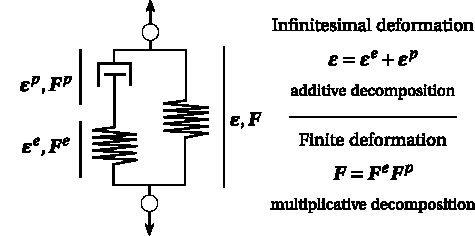
\includegraphics{figures/gradient_decomp}
	\caption{Additive and multiplicative strain decomposition corresponding to infinitesimal and finite deformations, respectively.}
\label{fig:gradient_decomp}
\end{figure}

Focusing on a decomposition between an elastic, denoted here by $e$, and a viscous element, denoted here by $p$, the application of the decomposition in Equation~\eqref{eq:mult_gradient_decomp} to the definition of the spatial velocity gradient yields
\begin{equation}
	\mathbf L = \mathbf L^e + \mathbf F^e \mathbf L^p (\mathbf F^e)^{-1},
\end{equation}
where $\mathbf L^e$ and $\mathbf L^p$ are defined as
\begin{align}
	\mathbf L^e =&  \do{\mathbf F}^e(\mathbf F^e)^{-1},\\
	\mathbf L^p =&  \do{\mathbf F}^p(\mathbf F^p)^{-1}.
\end{align}
The constitutive description is most often supplied as a law for $\mathbf D^p$ and $\mathbf W^p$, where
\begin{equation}
	\mathbf D^p = \operatorname{sym}(\mathbf L^p),\quad \mathbf W^p = \operatorname{skew}(\mathbf L^p).
\end{equation}
A common approach is \citep{desouzanetoComputationalMethodsPlasticity2008}
\begin{align}
  \label{eq:rate_plasticity_de_souza}
	\bar{\mathbf D}^p &\equiv  {\mathbf R^e}^T \mathbf D^p \mathbf R^e  = \dot\gamma_\text{dev} \mathbf N_\text{dev} + \dot\gamma_\text{vol} \mathbf N_\text{vol},\\
	\bar{\mathbf W}^p &\equiv {\mathbf R^e}^T \mathbf W^p \mathbf R^e = \bm 0,
\end{align}
with $\mathbf R^e$ defined by the polar decomposition theorem as $\mathbf F^e = \mathbf R^e\mathbf U^e$.
This yields for the plastic spatial velocity gradient
\begin{equation}
	\mathbf L^p = {\mathbf R^e}^T(\dot\gamma_\text{dev} \mathbf N_\text{dev} + \dot\gamma_\text{vol} \mathbf N_\text{vol})\mathbf R^e,
\end{equation}
and for elastic spatial velocity gradient
\begin{equation}
	\mathbf L^e = \mathbf L - (\dot\gamma_\text{dev} \mathbf N_\text{dev} + \dot\gamma_\text{vol} \mathbf N_\text{vol}).
\end{equation}
An alternative description can be given as
\begin{equation}
  \label{eq:flow_rule_lie_derivative}
	\frac{1}{2}£_v \mathbf b^e = -(\dot\gamma_\text{dev} \mathbf N_\text{dev} + \dot\gamma_\text{vol} \mathbf N_\text{vol})\mathbf b^e,
\end{equation}
where $£_v \mathbf b^e$ is the Lie derivative of $\mathbf b^e$ with respect to the velocity field $\bm v$.

One can also and prescribe $\mathbf D^p$, directly, \citep{boyceLargeInelasticDeformation1988},
\begin{align}
\label{eq:d_w_directly}
	\mathbf D^p & = \dot\gamma_\text{dev} \mathbf N_\text{dev} + \dot\gamma_\text{vol} \mathbf N_\text{vol},\\
	\mathbf W^p & = \bm 0,
\end{align}
or follow Bergström \citep{bergstromMechanicsSolidPolymers2015}
\begin{align}
	\label{eq:d_w_bergstrom}
	\tilde{\mathbf D}^p &\equiv \operatorname{sym}((\mathbf F^e)^{-1}\mathbf L^p \mathbf F^e) = \dot\gamma_\text{dev} \mathbf N_\text{dev} + \dot\gamma_\text{vol} \mathbf N_\text{vol},\\
	\tilde{\mathbf W}^p &\equiv \operatorname{skew}( (\mathbf F^e)^{-1}\mathbf L^p \mathbf F^e) = \bm 0,
\end{align}
which is equivalent to Equation~\eqref{eq:rate_plasticity_de_souza} assuming elasto-plastic isotropy, due to the coaxiallity of the flow rule and the right stretch tensor \citep{desouzanetoComputationalMethodsPlasticity2008}.

\subsection{Inclusion of the thermal field}
\label{sec:inclusion_thermal_field}

To take into account the the thermal field when employing constitutive descriptions based on rheological models, the mere inclusion of temperature dependent material parameters is not enough.
The first missing feature of such a model would be that a change in temperature, with null stress would not lead to a contraction or dilation, and by the same token a change in temperature while preventing expansion/contraction would lead to zero stress.
To fix this omission, an additional thermal configuration can be considered.
For example,
\begin{equation}
	\mathbf F = \mathbf F^\text{mech}\mathbf F^\text{th}.
\end{equation}
Note that the reverse order for the deformation gradients can be considerd, as well as, decompositions where the thermal deformation gradient is applied between elastic and plastic deformation gradients \citep{arrudaEffectsStrainRate1995}.

Reasoning about the models described so far, in a situation where the temperature increases, there is no stress response from the "mechanical part", thus its corresponding deformation gradient will be unitary, making the total deformation gradient equal to the thermal deformation gardient, $\mathbf F = \mathbf F^\text{th}$.
Taking inspiration from infinitesimal thermoelastic theory, one can write
\begin{equation}
	\label{eq:thermal_expansion_simple}
	\mathbf F^\text{th} = (1 + \alpha(T)\Delta T)\mathbf I.
\end{equation}
Lu and Pister \citep{luDecompositionDeformationRepresentation1975} suggest, however,
\begin{equation}
	\mathbf F^\text{th} = \upsilon(T)\mathbf I,
\end{equation}
where $\upsilon$ is a scalar-valued function of temperature, reflecting intrinsic thermal expansion characteristics of the material of the body
\begin{equation}
	\label{eq:expansion_function}
	\upsilon(T) = \exp\left[\int_{T_0}^T \alpha(T^*)\ dT^*\right],
\end{equation}
where $\alpha$ is coefficient of linear thermal expansion, allowed to depend on the temperature.
In particular, if $\alpha$ is independent of temperature, Equation~\ref{eq:expansion_function} reduces to
\begin{equation}
	\upsilon(\Delta T) = \exp(\alpha \Delta T).
\end{equation}
Furhter, if the conditions for infinitesimal thermal strain are satified, i.e., $\alpha\Delta T \ll 1$, one finds Equation~\eqref{eq:thermal_expansion_simple}.

Taking a look at the energy balance equation (Equation~\eqref{eq:heat_conduction}), two elements are still missing from the present analysis: the internal dissipation and Gough-Joule effect.
In the one-dimensional rheological model, the dissipation is due to the linear dashpots,
\begin{equation}
	\mathcal D^i_\text{int} = \sigma^i {\dot\gamma}^i,
\end{equation}
where ${\dot \gamma}^i$ is the strain rate the dashpot $i$ is subject to and $\sigma^i$ is the stress across the same element.
In three-dimensions, this is rational yields
\begin{equation}
	\mathcal D_\text{int}^i = \chi_\text{d}\mathbf \sigma_i : \mathbf D^i,
\end{equation}
where $\bm \sigma^i$ is the Cauchy stress tensor across the $i$th viscous elements and $\mathbf D^i$ the corresponding rate of deformation tensor.
$\chi_\text{d}\in [0, 1]$ is a constant dissipation factor, commonly chosen in the range $\chi_\text{d}\approx 0.85$ to 0.95 for metals \citep{simoAssociativeCoupledThermoplasticity1992} and equal to 1 for polymers \citep{okerekeTwoprocessConstitutiveModel2019, haoRatedependentConstitutiveModel2022}.
The possibility of $\chi_\text{d}<1$ materializes the fact that some plastic work may be stored in the material.

The thermoelastic Gough-Joule effect can be written as
\begin{equation}
	\mathcal H^\text{e} = -\rho_0T\frac{\partial \mathbf P}{\partial T}:\dot{\mathbf F},
\end{equation}
discarding the contribution from the dissipation, following Simo and Mihe \citep{simoAssociativeCoupledThermoplasticity1992}--compare with the full equation for the elatoplastic Gough-Joule effect (Equation~\eqref{eq:def_gough_joule_effect}).

The considerations given in this section are rendered useless if the model is formulated employing a free energy which depends also on the temperature, e.g., those models described in  \citep{anandThermomechanicallyCoupledTheory2009, amesThermomechanicallyCoupledTheory2009}.

\subsection{Models available in the literature}
\label{sec:rheo_models}
% \colorbox{BrickRed}{See connection with rate independent plasticity. \citep{naghdiMechanicalBehaviorViscoelastic1963}}

% \colorbox{BrickRed}{Mention the work of Kauzmann an Eyring \citep{kauzmannViscousFlowLarge1940} and discussed constant structure.}

The next set of models corresponds to generalizations of various infinitesimal viscoelastic models through the use of the previously described non-linear elements in place of the linear elements in the corresponding rheological models.

\paragraph{Generalization of the Maxwell model}
The Maxwell model is given as
\begin{equation}
	\sigma + \frac{\eta}{E}\dot \sigma = \eta \dot \varepsilon,
\end{equation}
corresponding to the rheological model in Figure~\ref{fig:rheo_model_maxwell}.
\begin{figure}
	\centering
	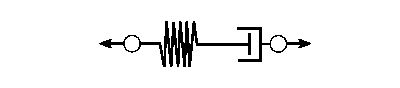
\includegraphics{figures/rheo_model_maxwell}
	\caption{Rheological model corresponding to the Maxwell model.}
\label{fig:rheo_model_maxwell}
\end{figure}
An early improvement with the goal of describing the large-strain behavior of elastormers is presented by Smith \citep{smithNonlinearViscoelasticResponse1962}.
The Bodner-Partom material model \citep{bodnerConstitutiveEquationsElasticViscoplastic1975} is another generalization of the same constitutive description.
It can simulate the behavior of a visco-elasto-plastic material under small strains and arbitrary loading history.
The elastic element obeys Hooke's law and the flow rule is given according to Equations~\eqref{eq:d_w_directly} and \eqref{eq:exp_flow_law} with the athermal strength evolving according to Equation~\eqref{eq:bodner_partom_rate_eq}.
% \begin{align}
% 	\dot\gamma_\text{dev} &= \sqrt{2} D_0 \exp\left(-\frac{1}{2}\left(\sqrt{2}\frac{\hat \tau}{\|\mathbf s\|}\right)^n\right),\\
% 	\dot\gamma_\text{vol} &= 0
% \end{align}
% where $\hat \tau$ is defined according to
% \begin{equation}
% 	{\hat \tau}^2 = \frac{1}{3}Z^2 \left(\frac{n+1}{n}\right)^{1/n},
% \end{equation}
% and $D_0$,  $n$ and $Z$ are material properties with the former taken as an internal variable following the rate equation
% \begin{equation}
% 	\label{eq:rate_equation_exp}
% 		\dot Z = m\left(\frac{Z_1 - Z}{Z_0}\right)\dot w_p,
% \end{equation}
% where $Z_0$, $Z_1$ and $m$ are also material properties and $w^p$ is the plastic work, i.e.,
% \begin{equation}
% 	w^p \equiv \int_0^t \bm \sigma : \mathbf D^p\ d\tau.
% \end{equation}
% Equation~\eqref{rate_equation_exp} can be integrated explicitly yielding
% \begin{equation}
% 	Z = Z_1 + (Z_0 - Z_1)\exp\left(-\frac{m}{Z_0}w^p\right).
% \end{equation}
% See Figure~\ref{fig:internal_var_exp} for the plot.
The model is capable of describing a rate sensitive response and hardening, however it cannot display strain recovery.
Based in this work, the rate equations in Equation~\eqref{eq:rate_eq_zairi} for $\hat \tau$ in a power law (see Equation~\eqref{eq:flow_rule_power_law}) have been used in models describing poly(methyl methacrylate) (PMMA), a glassy polymer, by Zaïri and co-workers \citep{zairiPhenomenologicalNonlinearModelling2005, zairiElastoviscoplasticConstitutiveEquations2007,zairiModellingElastoviscoplasticDamage2008}, to describe HDPE by Zhang and Moore \citep{zhangNonlinearMechanicalResponse1997}, and to describe PC by Frank and Brockman \citep{frankViscoelasticViscoplasticConstitutive2001}.
It has also been used to model the behavior of metallic alloys at high temperatures \citep{desouzanetoComputationalMethodsPlasticity2008}.
% \begin{figure}
% 	\centering
% 	\includegraphics[widht=0.9\textwidth]{example-image-a}
% 	\caption{Evolu}
% \end{figure}

In the same vein, Ben Hadj Hamouda et al. \citep{benhadjhamoudaViscoplasticBehaviourMedium2007} employ a Double Inelastic Deformation (DID) model---whose background is described in detail by Cailletaud and Saï \citep{cailletaudStudyPlasticViscoplastic1995}.
It is formulated in small strains and an additive split is assumed between a linear strain and two viscoplastic strains, corresponding to the different deformation mechanism in the amorphous and crystalline phases.
Each viscoplastic strain follows a power law (see Equation~\eqref{eq:flow_rule_power_law}) with a von Mises yield criterion, accounting also for kinematic nonlinear hardening.
%  according to
% \begin{align}
% 	\bm \beta_i &= \bm \alpha_i\\
% 	\dot{\alpha}_i &= \bm \varepsilon_{vp,i} + \bm \beta_i\dot\gamma_{\text{dev},i},
% \end{align}
% where $\bm \beta$ is a backstress tensor, a $\bm \varepsilon_{vp}$ is a viscoplastic infinitesimal strain and the subscript $i=1,2$ corresponds to the different viscoplastic strain identified with each of the phases.
It is used by the authors to model the response of MDPE to constant strain rate uniaxial traction experiments, as well as stress relaxation and dip tests.
Balieu et al. \citep{balieuNonassociatedViscoplasticityCoupled2014} also present a model that can be interpreted as a non-linear Maxwell model.
It is formulated employing hypoelasticity, with the plastic flow rule deduced from Raghava's criterion modified to include an isotropic damage variable representing the micro-voids and micro-cracks that develop in the material.
The law for the strain rate is a power law (see Equation~\eqref{eq:flow_rule_power_law}) and the authors employ an integral-type nonlocal damage model to describe mineral filled semi-crystalline polymers.

\paragraph{Standard Linear Solid}
The following set of models are generalizations of the so-called standard linear solid model.
In the context of infinitesimal viscoelasticity it can be expressed in equivalent ways in its Maxwell or its Kelvin-Voigt representation, as shown in Figure~\ref{fig:rheo_model_sls} with the constitutive differential equations for the stress and the strain given as
\begin{gather}
	\sigma+\frac{\eta}{E_2} \dot{\sigma}=E_1 \varepsilon+\frac{\eta\left(E_1+E_2\right)}{E_2} \dot{\varepsilon},\quad\text{(Maxwell representation)},
	\label{eq:sls_maxwell_rep}\\
	\sigma+\frac{\eta}{E_1+E_2} \dot{\sigma}=\frac{E_1 E_2}{E_1+E_2} \varepsilon+\frac{E_1 \eta}{E_1+E_2} \dot{\varepsilon},\quad\text{(Kelvin-Voigt represenation)},
	\label{eq:sls_voigt_rep}
\end{gather}
where in both equations the terms containing the strain, $\varepsilon$, are the stress response in equilibrium.
\begin{figure}[hbtp]
\centering
\begin{subfigure}[b]{0.45\textwidth}
\centering
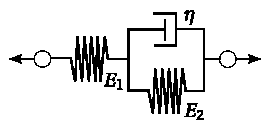
\includegraphics[width=\textwidth]{figures/rheo_model_sls_maxwell}
\caption{}
\label{subfig:rheo_model_sls_maxwell}
\end{subfigure} \hfill
	\begin{subfigure}[b]{0.45\textwidth}
		\centering
						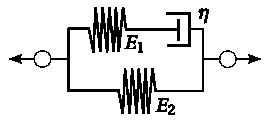
\includegraphics[width=\textwidth]{figures/rheo_model_sls_voigt}
						\caption{}
						\label{subfig:rheo_model_sls_voigt}
		\end{subfigure}
	\caption{Rheological model for the standard linear solid. \subref{subfig:rheo_model_sls_maxwell} Maxwell representation. \subref{subfig:rheo_model_sls_voigt} Voigt representation.}
\label{fig:rheo_model_sls}
\end{figure}

The viscoplasticity theory based on overstress (VBO) was introduced by Cernocky and Krempl \citep{cernockyTheoryViscoplasticityBased1980} and is based on the standard linear-solid.
The so-called overstress is the difference between the full stress and the equilibrium part, which is allowed to be a nonlinear function of the strain.
Thus, Equation~\eqref{eq:sls_maxwell_rep} and \eqref{eq:sls_voigt_rep} can be written as
\begin{equation}
	\sigma - f(\varepsilon) = M\dot\varepsilon - K\dot \sigma,
\end{equation}
where $f$ may be a nonlinear function of the strain, and $M$ and $K$ are general functions of the stress, the strain and their derivatives.
It has been used to successfully model metals \citep{liuUniaxialViscoplasticModel1979, yaoViscoplasticityTheoryBased1985}, as well as, polymers, such as polypropylene \citep{kitagawaRatedependentNonlinearConstitutive1989}, polyethylene \citep{kitagawaNonlinearConstitutiveEquation1990}, nylon 66, polyetherimide, poly(ether ether ketone) \citep{krempl2000overstress}, or polyphenylene oxide (PPO) \citep{colakModelingDeformationBehavior2005}.
More advanced versions of this approach include kinematic and isotropic hardening, as well as, strain softening through the use of appropriate internal variables \citep{krempl2000overstress, hoExtensionViscoplasticityTheory2002}.

The generalization to large strains and three dimensions of the Maxwell or the Voigt-Kelvin representation of the standard linear solid may not be equivalent.
Concerning the generalization of the Maxwell representation, Simo \citep{simoFullyThreedimensionalFinitestrain1987} and Reese and Govindjee \citep{reeseTheoryFiniteViscoelasticity1998} consider non-linear elastic elements in the rheological model.
The first author employs the analytical solution for the ordinary differential equations describing the standard linear solid model yielding a representation for the isochoric part of the stress as a convolution integral, i.e.,
\begin{align}
	\mathbf S &= Jp\mathbf C^{-1} + J^{-2/3}\operatorname{dev}[\mathbf H],\\
	\mathbf H &= \int_0^t (\gamma + (1-\kappa)e^{-(t-\tau)/T}) \frac{d}{d\tau}\left\{\operatorname{dev} \left[\frac{\partial {\bar\psi}_\text{EQ}(\bar{\mathbf E}(\tau))}{\partial \bar{\mathbf E}}\right]\right\}  d\tau,
\end{align}
where $\kappa$ is a parameter such that $\kappa=0$ coincides with the Maxwell model for the isochoric part of the stress and $\kappa=1$ to the elastic solid, $\theta$ is the relaxation time, $\bar{\bm E}$ is the Green-Lagrange strain tensor computed from the volume-preserving part of the deformation gradient $\bar{\bm F} \equiv J^{-1/3} \bm F$, and $\bar{\psi	}_\text{EQ}$ is the equilibrium term in the free energy.

On the other hand, Reese and Govindjee \citep{reeseTheoryFiniteViscoelasticity1998}, opt for a rate equation for the elastic left Chauchy-Green strain tensor coinciding with a Newtonian fluid (see Equation~\eqref{eq:newton_fluid_flow_rule_norm} and \eqref{eq:flow_rule_lie_derivative}), employing a multiplicative split for the deformation gradient.
Accordingly, the second Piola-Kirchhoff stress tensor is given as
\begin{equation}
	\mathbf{S}=\mathbf{S}_{E Q}+\mathbf{S}_{N E Q}=\underbrace{2 \frac{\partial \psi_{E Q}}{\partial \mathbf{C}}}_{\mathbf{S}_{E Q}}+\underbrace{2 (\mathbf{F}^i)^{-1} \cdot \frac{\partial \mathbf{\psi}_{N E Q}}{\partial \mathbf{C}^e} \cdot (\mathbf{F}^i)^{-T}}_{\mathbf{S}_{N E Q}}=2 \frac{\partial \psi}{\partial \mathbf{C}},
\end{equation}
where $\mathbf S_\text{EQ}$ and $\mathbf S_\text{NEQ}$ are the stresses corresponding to equilibrium and non-equilibrium, respectively.
Appropriate choices for the free energy $\Psi$ yield different nonlinear elastic elements.

Polanco-Loria et al. \citep{polanco-loriaConstitutiveModelThermoplastics2010} present their generalization which allows for hyperelastic-viscoplastic response due to intermolecular resistance and entropic hyperelastic response due to re-orientation of molecular chains.
The stress in the Maxwell arm is given according to the isotropic compressible Neo-Hookean material (see Equation~\eqref{eq:neo_hookean_model}), while the flow in the dashpot is controled by Raghava's yield criterion, which is pressure sensitive (see Section~\ref{sec:yield_criteria}).
A non-associative viscoplastic flow potential is employed, allowing for volumetric plastic strain.
Finally, the deviatoric part of the stress on the other arms is given by the eight-chain model, including also a volumetric part similar to the one shown in Equation~\eqref{eq:neo_hookean_model} for the Neo-Hookean model.
The authors validated their models against experimental results obtained for polypropylene samples.

However, perhaps the most popular thermoplastic models are generalizations of the Voigt version of the standard solid.
Halsey et al. \citep{halseyMechanicalPropertiesTextiles1945} present one of the earliest contributions considering an Eyring dashpot as the viscous element in an attempt to model the behavior of fibers.
Likewise, Haward and Thackray \citep{hawardUseMathematicalModel1968} proposed one of the first models for thermoplastic polymers below the glass transition temperature.
The elastic element $A$ is still a linear spring, however, the elastic element $B$ is a Langevin spring, while the viscous element parallel to it is an Eyring dashpot.
The model is formulated assuming small strains and is restricted to one-dimensional loading.

Later, Boyce et al. \citep{boyceLargeInelasticDeformation1988} generalized this model to three-dimensions, among other additions.
A multiplicative kinematic split between the elastic and inelastic deformation is enforced, as described in Section~\ref{sec:generalization_large_strains_3d}.
The elastic spring $A$ is generalized to three dimensions and large deformation employing the Hencky model (see Equation~\eqref{eq:hencky_model}), with shear and bulk modulus being temperature dependent.
The thermally activated process is now nucleation controlled employing the aforementioned model by Argon \citep{argonTheoryLowtemperaturePlastic1973} (see Equation~\eqref{eq:argon_model_free_enthalpy}) with the addition that the athermal strength $s_0$ is replaced by an internal variable, $\tilde s$, which is given by $\tilde{s}=s+\alpha p,$ where $p=-\sigma_m$ and $\alpha$ is a material property.
The rate equation for the athermal strength, $s$, is chosen according to Equation~\eqref{eq:rate_equation_bpa}, such that the distinctive strain softening of glassy polymers is captured.
The model does not account for volumetric flow.
Lastly, the stress in the elastic element $B$ is given by the three-chain model in (see Equation~\eqref{eq:three_chain_model}).
For other contributions exploring this model while employing different rubber-like elasticity models see, e.g., \cite{arrudaEvolutionPlasticAnisotropy1993, arrudaEffectsStrainRate1995, wuImprovedNetworkModels1993, buckleyGlassrubberConstitutiveModel1995, sweeneyRateDependentNetwork1995}.
In fact the most widely used model of this type is the so-called Arruda-Boyce model \citep{arrudaEvolutionPlasticAnisotropy1993, arrudaEffectsStrainRate1995}, which employs an eight-chain model for the elastic element $B$.

Also expanding on the model of Boyce, Parks and Ahzi \citep{boyceLargeInelasticDeformation1988} (BPA model), Chowdhury et al. \citep{chowdhuryEffectsManufacturingInducedVoids2008} propose in the context of manufacturing-induced voids in polymer-based composites a very similar model, formulated however hypoelastically.
The model was later validated on epoxy resins by Poulain et al. \citep{poulainFinitestrainElastoviscoplasticBehavior2014}.
As in the BPA model, the athermal strength (Equation~\eqref{eq:argon_model_free_enthalpy}) is taken as an internal variable following, however, a different rate equation (Equation~\eqref{eq:two_athermal_strength_evo}).
This choice allows a smoother strain softening.
Also, the response of the elastic element $B$ is now a linear combination of the response obtained from a three-chain model (Equation~\eqref{eq:three_chain_model}) and an eight-chain model (Equation~\eqref{eq:eigth_chain_model}).
Hao et al. \citep{haoUnifiedAmorphousCrystalline2022} propose a very similar model, where however the rate equation for the athermal strength is given by Equation~\eqref{eq:rate_equation_hao}, rendering a model able to capture the double yield phenomenon in semi-crystalline polymers.
The last authors also take into account the thermomechanical aspects of polymer modeling accounting for the self-heating, thermal softening and temperature dependent properties.
They validate their model against experimental results obtained on epoxy, nylon10 and PA6.

\paragraph{Burgers material}
Another common material model in infinitesimal viscoelasticity is the so-called Burgers material, which incorporates viscous flow into the standard linear solid model.
It also accepts two equivalent descriptions as
\begin{gather}
	\sigma+\left(\frac{\eta_1}{E_1}+\frac{\eta_2}{E_2}\right) \dot{\sigma}+\frac{\eta_1 \eta_2}{E_1 E_2} \ddot{\sigma}=\left(\eta_1+\eta_2\right) \dot{\varepsilon}+\frac{\eta_1 \eta_2\left(E_1+E_2\right)}{E_1 E_2} \ddot{\varepsilon}\quad \text{(Maxwell representation)},\\
	\sigma+\left(\frac{\eta_1}{E_1}+\frac{\eta_2}{E_1}+\frac{\eta_2}{E_2}\right) \dot{\sigma}+\frac{\eta_1 \eta_2}{E_1 E_2} \ddot{\sigma}=\eta_2 \dot{\varepsilon}+\frac{\eta_1 \eta_2}{E_1} \ddot{\varepsilon}\quad \text{(Kelvin-Voigt representation)},
\end{gather}
in the context of small strains.
See Figure~\ref{fig:rheo_model_burgers} for the corresponding rheological models.
\begin{figure}
\centering
\begin{subfigure}[b]{0.57\textwidth}
\centering
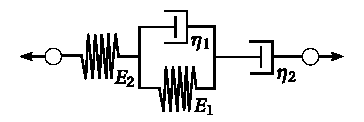
\includegraphics[width=\textwidth]{figures/rheo_model_burgers_maxwell}
\caption{}
\label{subfig:rheo_model_burgers_maxwell}
\end{subfigure} \hfill
	\begin{subfigure}[b]{0.42\textwidth}
		\centering
						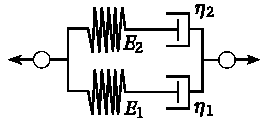
\includegraphics[width=\textwidth]{figures/rheo_model_burgers_voigt}
						\caption{}
						\label{subfig:rheo_model_burgers_voigt}
		\end{subfigure}
  \caption{Rheological model for the Burgers material. a) Maxwell representation. b) Voigt representation.}
  \label{fig:rheo_model_burgers}
\end{figure}

Bardenhagen et al. \citep{bardenhagenThreedimensionalFiniteDeformation1997} propose a three-dimensional viscoplastic model for polymeric materials which is a generalization of the Maxwell representation of the Burgers material.
One of the arms is a three-dimensional large strain hypoelastic generalization of the Maxwell model.
The other arm employs a associatiave hypoelastic elasto-plastic model with the von Mises criterion as the yield criterion.
It includes isotropic hardening function of the plastic flow rate, and comparison with experimental results.

Boyce et al. \citep{boyceConstitutiveModelFinite2000} also present a model generalizing the Maxwell representation of the Burgers material.
One of the arms contains an elastic elements following Hencky's model (see Equation~\eqref{eq:hencky_model}) and an Eyring dashpot in the same way as the model already described found in \citep{boyceLargeInelasticDeformation1988}.
In other arm the elastic element follows the eight-chain model (see Equation~\eqref{eq:eigth_chain_model}), while the dashpot is similar to the Bergström-Boyce model (see Equation~\eqref{eq:bb_reptation_model}).
It is used by the authors to model poly(ethylene terephthalate) above the glass transition temperature accounting for strain-induced crystallization.
This is achieved neglecting dashpot $D$ if the stretch is larger than a given value, which depends on the plastic strain rate and the temperature.

Kletschkowski et al. \citep{kletschkowskiEndochronicViscoplasticMaterial2002} present another description fitting into this class of material models.
One of the Maxwell arms is made of a linear elastic spring and its viscous element follows the cooperative model (see Equation~\eqref{eq:cooperative_flow_rule}) for the strain rate.
The other arm employs the endochronic viscoplasticity theory \citep{valanisTheoryViscoplasticityYield1970}.
It resembles viscoelasticity with the caveat that time is replaced by an "inner" time, function of the strain, hence the name endochronic.
The authors employ this model in the description of filled PTFE.

Pouriayevali et al. \citep{pouriayevaliConstitutiveDescriptionRatesensitive2013} present a constitutive model to describe the quasi-static and high strain rate, large deformation response of semi-crystalline polymers, which can be seen as generalization of the Kelvin-Voigt representation of the Burgers material.
The elastic elements are hyperelastic and their stress response is obtained from Equation~\eqref{eq:constitutive_equation_stress_thermoelasticity} given a suitable free energy potential.
Regarding the viscous elements, element $A$ obeys von Mises yield criterion with the strain rate also given by Equation~\eqref{eq:flow_rule_perzyna} and element $B$ obeys Newton's viscosity law (see Equation~\eqref{eq:newton_fluid_flow_rule}) neglecting the volumetric contribution.
The corresponding free energy, including the dependency on the temperature is also supplied.
The authors validate their model through comparisons with Nylon 6.

The dual network fluoropolymer model is presented in \cite{bergstromConstitutiveModelPredicting2005} as an extension of the Bergström and Boyce \citep{bergstromConstitutiveModelingLarge1998} and Arruda and Boyce model \citep{arrudaEffectsStrainRate1995}, generalizing the Kelvin-Voigt representation of the Burgers material.
The response of both springs is given by the Arruda-Boyce eight-chain model (see Equation~\eqref{eq:eigth_chain_model}), with the response of the element $B$ taken as a scalar factor $s_B$, a specified material parameter, times the expression employed to describe the response of the element $A$ evaluate according to the deformation gradient accross $B$.
The kinematic decomposition is as expected from the discussion in Sections~\ref{sec:generalization_large_strains_3d} and \ref{sec:inclusion_thermal_field} including a thermal deformation gradient.
The rate equations for $\dot\gamma^C_\text{dev}$ and $\dot\gamma^C_\text{vol}$ in Equation~\eqref{eq:d_w_bergstrom} for the viscous element $C$ is given similarly to the Bergström-Boyce model (see Equation~\eqref{eq:bb_reptation_model}) multiplied by a power laws function of the stress and the temperature.
The volumetric strain rate is given according to Equation~\eqref{eq:newton_fluid_flow_rule_norm}.
The strain rate for the viscous element $D$, $\dot \gamma^D_\text{dev}$, is given by
\begin{equation}
	\dot{\gamma}_\text{dev}^D=\begin{cases}
	a b\left(\varepsilon-\varepsilon_0\right)^{b-1} \dot{\varepsilon} & \text { if } \tau>\sigma_0 \\
	0 & \text { otherwise }
	\end{cases},
\end{equation}
where $\varepsilon = \|\mathbf E^{(0)}\|$, $a >0$, $b>0$ and $\sigma>0$ are material parameters, $\tau = \|\mathbf s\|$, which is similar to a von Mises yield criterion.
% \colorbox{BrickRed}{Consider also the contribution of \cite{khanFiniteDeformationPolymer2001}}

\paragraph{Generalized Maxwell model}
A generalized Maxwell model is one that contains $n$ Maxwell arms in parallel.
In addition, a single arm with only an elastic element may also be considered.
See Figure~\ref{fig:rheo_model_gen_maxwell} for the corresponding rheological models.
This framework includes both Maxwell representations for the standard linear solid model and the Burgers material.
Models with more than two arms are considered in the following section.
\begin{figure}[htbp]
	\centering
	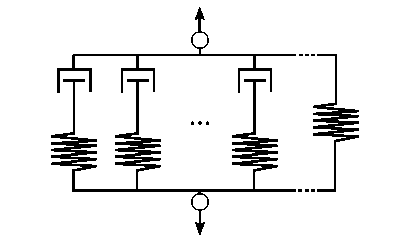
\includegraphics{figures/rheo_model_gen_maxwell}
	\caption{Rheological model for the generalized Maxwell model.}
\label{fig:rheo_model_gen_maxwell}
\end{figure}

Holmes et al. \citep{holmesConstitutiveModelLarge2006} present a large strain deformation elasto-viscoplastic material model for the modeling of semi-crystalline polymers.
According to the authors each of the arms in the model coincides with a mode of deformation, elastic, viscoelastic and viscoplastic.
The response of each the elastic elements follows from a free energy and the constitutive relation in Equation~\eqref{eq:constitutive_equation_stress_thermoelasticity}.
The suggestion left by the authors is to employ an Ogden potential for the elastic and viscoelastic arms, and a Saint Venant-Kirchhoff potential (see Equation~\eqref{eq:saint_venant_kirchhoff}) for the viscoplastic contribution.
The flow rule adopted follows the work of
% for viscoelastic arm of the model is given according to Equation~\eqref{eq:} with $\eta_\text{vol}=0$ and
% \begin{equation}
% 	\eta_\text{dev}=\frac{h_0-h_1 \exp \left\{h_2 \frac{\left|\vec{\varepsilon}^e\right|+3 \times 10^{-5}}{\left|\tilde{\varepsilon}^i\right|}\right\}-h_3 \exp \left\{h_4 \frac{\left|\dot{\varepsilon}^e\right|+3 \times 10^{-5}}{\left|\dot{\varepsilon}^i\right|}\right\}}{\left(\left|\dot{\varepsilon}^e\right|+3 \times 10^{-5}\right)^{n e}},
% \end{equation}
% where $h_{0,1,\dots,4}$ and $ne$ are material constants.
Brussele-Dupend et al. \citep{brusselle_dupendMechanical2001, brusselle_dupendMechanical2003} for semi-crystalline polypropylene, accounting for the inadequecis of the Eyring equation (see Equation~\eqref{eq:eyring_model}).
Regarding the viscoplastic arm of the model, the strain rate is given according to Equation~\eqref{eq:flow_rule_directions} and \eqref{eq:flow_rule_perzyna}.

% according to an associative description employing the von Mises criterion and strain rate given by
% \begin{equation}
% \label{eq:perzyna}
% \dot\gamma_\text{dev, vp} = R\left(\|\mathbf s_\text{vp} + \bm \beta\| - \sqrt{\frac{2}{3}}(\sigma_Y - q)\right),
% \end{equation}
% where $R$ is the ramp function, $\bm \beta$ is the backstress, $\sigma_Y$ is the yield strength and $q$ is an isotropic hardening internal variable.


% \colorbox{BrickRed}{Include a brief mention of the work of \cite{zerilliConstitutiveEquationDynamic2007}}


Zeng et al. \citep{zengConstitutiveModelSemicrystalline2010} developed an elastoplasticity constitutive model for semi-crystalline polymers in the framework of isothermal conditions, between the glass transition temperature and the melting temperature under low-level strain rates, neglecting viscous effects.
Each of the arms in the rheological model is based on physical considerations concerning the mesoscopic semi-crystalline structure.
The foundational idea is that of a three-phase morphology depending on the average distance between crystalline blocks.
When the distance is small the interaction is modeled as being elastoplastic with linear hardening.
For medium distances, the behavior is elastoplastic with perfect plasticity, and for large distance, the material is modeled as following the eight chain model (see Equation~\eqref{eq:eigth_chain_model}).
The authors validated the model against the results of uniaxial and biaxial experiments on polyamide 6 and polyethylene at different strain rates.
The model parameters are easily calibrated using these uniaxial stress–strain experimental curves.

% \colorbox{BrickRed}{See also \cite{buckleyGlassrubberConstitutiveModel1995}}
Okereke and Akpoyomare \citep{okerekeTwoprocessConstitutiveModel2019} propose a model based on an elastic-viscoelastic-viscoplastic framework, to predict the temperature and rate-dependent response of an incompressible semi-crystalline polymer.
It is materialized by three arms in a rheological model, two containing a viscous and an elastic element corresponding to the contribution of the mobile amorphous fraction; and the crystalline and rigid amorphous fractions, and another arm containing only an elastic element, representing the contribution of the entangled molecular network.
The basis of this model is a one-process glass-rubber model for amorphous polymers \citep{buckleyGlassrubberConstitutiveModel1995}, which is adapted to the description of semi-crystalline polymers considering the $\alpha$- and the $\beta$-processes, making it a two-process model.
These processes are connected by the authors to the glass transition of the rigid amorphous and the mobile amorphous phases, respectively.
The flow rule for both arms containing the viscous elements is given according to Equation~\eqref{eq:flow_rule_directions}, where the volumetric contribution is neglected and the deviatoric strain rate is given by
\begin{equation}
	\dot \gamma_\text{dev, i} = \dot \gamma_{T,j}\dot\gamma_{S,j}\dot\gamma_{\sigma,j}\dot\gamma_{0,j},\quad j=\alpha, \beta
\end{equation}
where $\dot \gamma_{T,j}$ captures the influence of the temperature as
\begin{equation}
	\dot \gamma_{T,j} = \exp\left(-\frac{\Delta H_j}{k_B T}\right),
\end{equation}
and $\dot \gamma_{\sigma,j}$ captures the influence of the stress as
\begin{equation}
	\dot\gamma_{\sigma,j} = \exp\left(\frac{\Omega\sigma_m}{k_B T}\right)\sinh\left(\frac{v\|\mathbf s\|}{2\sqrt{3}k_BT}\right),
\end{equation}
according to Eyring's theory (see Equations~\eqref{eq:eyring_model} and \eqref{eq:eyring_w_pressure}).
The influence of the structure is taken into account through a fictive temperature $T_f$ for each arm $j$ as
\begin{equation}
	\dot\gamma_{S,j} = \exp\left(\frac{C}{T_{f,j}-T_\infty}\right),
\end{equation}
where $C$ is the Cohen-Turnbull constant and $T_\infty$ is the Vogel temperature.
The pre-exponential factor is given by
\begin{equation}
	\dot \gamma_{0,j} = \frac{G}{\tau^*_{0,j}} \frac{v}{k_B T}\exp\left(\left[\frac{\Delta H}{R\Delta T}\right]\left[\frac{C}{\Delta T_{f,j} - T_\infty}\right]\right),
\end{equation}
where the superscript $*$ denotes a reference value and $\tau_0$ is a relaxation time.
The rate equation for the fictive temperature is given by
\begin{equation}
	\dot T_{f,j} = (T - T_{f,j})\dot\gamma_{S,j}\dot\gamma_{T,j}\dot\gamma'_{0,j} + \kappa \|\mathbf D^{p,j}\|,\quad j = \alpha, \beta,
\end{equation}
where $\kappa$ is a material parameter and
\begin{equation}
	\dot \gamma'_{0,j} = \frac{1}{\tau^*_{0,j}} \exp\left(\left[\frac{\Delta H}{R\Delta T}\right]\left[\frac{C}{\Delta T_{f,j} - T_\infty}\right]\right).
\end{equation}
This choice of the rate equation of the fictive temperature incorporates into the model significant post-yield strain-softening observed in high rate compression of propylene, according to the authors.
The elastic elements in the arms containing viscous elements according to the Saint-Venant-Kirchhoff model (see Equation~\eqref{eq:saint_venant_kirchhoff}), while the other elastic element follows the Edwards-Vilgis model (see Equation~\eqref{eq:edward_vilgis_model}).

The three network model is presented in \citep{bergstromMechanicsSolidPolymers2015}, being very similar to the models already presented based on a generalized Maxwell model.
The springs follow the Arruda-Boyce eight-chain model (see Equation~\eqref{eq:eigth_chain_model}) and the dashpots a power laws (similar to Equation~\eqref{eq:flow_rule_power_law}).
The effective shear stress is taken as an internal variable with a corresponding rate equation.
A linear dependence on the temperature for the stress response of the elastic elements is also included.
The same author also explores a parallel network model which consists in adding more Maxwell arms to the model following similar constitutive equations.

Hao et al. \citep{haoRatedependentConstitutiveModel2022} propose a model containing three arms, to study the double yield phenomenon as well as the rate- and temperature-dependent thermomechanical response below the glass transition temperature of semi-crystaline polymers.
The first arm contains an elastic element whose stress response follows Hencky's model (see Equation~\eqref{eq:hencky_model}).
The corresponding viscous element obeys Equations~\eqref{eq:eyring_model} and \eqref{eq:argon_model_free_enthalpy} following the work of Boyce et al. \citep{boyceLargeInelasticDeformation1988}.
The athermal strength is taken as an internal variables and its rate equation is shown in Equation~\eqref{eq:two_athermal_strength_evo}, following Chowdhury et al. \citep{chowdhuryEffectsManufacturingInducedVoids2008}.
The behavior of the elasto-plastic arm coincides with rate-independent plasticity and it is made up of an elastic element also following Hencky`s model (see Equation~\eqref{eq:hencky_model}) and a viscous element respecting a paraboloidal yield criterion.
The yield criteion describing the yield in the crystalline region is similar to the Drucker-Prager yield criteria with strain rate/plastic multiplier $\dot \gamma$ found taking into account the Kuhn-Tucker's loading-unloading consistency conditions.
The same law as Chowdhury et al. is adopted for the rubber-like elastic responsible for the hardening response, combining a  four-chain model (see Equation~\eqref{eq:three_chain_model}) and an eight-chain model (see Equation~\eqref{eq:eigth_chain_model}).

The hybrid model has been developed to model UHWPE \citep{bergstromConstitutiveModelingUltrahigh2002, bergstromPredictionMultiaxialMechanical2003} and employs the rheological model shown in Figure~\ref{fig:hybrid_model}.
The spring E is linear following th Hencky model (Equation~\eqref{eq:hencky_model}), springs A and B follow the Arruda-Boyce eight-chain model (Equation~\eqref{eq:eigth_chain_model}), employing the same expression with exception of a multiplicative constant $s_B$.
This constant is treated in the model as an internal variable which evolves according to an equation similar to Equation~\eqref{eq:bodner_partom_rate_eq}.
The rate of viscoplastic flow in the element $P$, $\dot\gamma^P$, is given by a power law (Equation~\eqref{eq:flow_rule_power_law}), as is the flow rate in the element $B$.
\begin{figure}[hbtp]
  \centering
	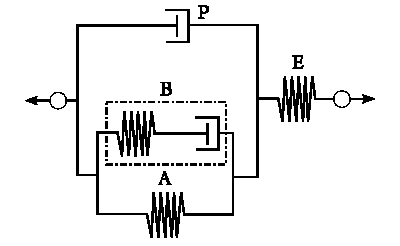
\includegraphics{figures/hybrid_model}
	\caption{Rheological representation of the Hybrid model \citep{bergstromConstitutiveModelingUltrahigh2002, bergstromPredictionMultiaxialMechanical2003}.}
\label{fig:hybrid_model}
\end{figure}

\section{Based on free energy}

Yet another approach is to postulate a free-energy wich depends both on the deformation gradient and the temperature, in addition to appropriate internal variables.
Providing suitable rate equations for these variables, one can fully specify the constitutive description of a polymer.
However, most of these models can be reinterpreted as generalizations of rheological modes as described in the previous section, employing much of the same laws already described.
For some examples see \cite{anandTheoryAmorphousSolids2003, ghorbelViscoplasticConstitutiveModel2008,anandThermomechanicallyCoupledTheory2009, amesThermomechanicallyCoupledTheory2009, pouriayevaliConstitutiveDescriptionRatesensitive2013}.

\section{Models considering bulk crystallinity}
\label{sec:models_bulk_crystal}

The following set of models considers different phases in the semi-crystalline polymers, a crystalline phase and an amorphous phase.
They do so through simple geometric considerations which mostly only include the bulk crystallinity.
The simplest results of this kind are the Voigt and Reuss mixture rules \citep{wardIntroductionMechanicalProperties2004}.
It is assumed that the two phases, $A$ and $B$, are disposed as layers (see Figure~\ref{subfig:voigt_mixture_rule}), with the Voigt rule obtained assuming that the strain is the same in all composite layers, yielding
\begin{equation}
	\label{eq:voigt_mixture_rule}
	E_\text{mix, Voigt} = E_A \chi + E_B (1 - \chi),
\end{equation}
for the modulus of the mixture, $E_\text{mix}$, with $E_A$ and $E_B$ the modulus of each phase, and $\chi$ the volume fraction of the phase $A$.
This rule sets an upper limit to the stiffness of the composite material.
If on the other hand, it is assumed that the stress is the same in all composite layers (see Figure~\ref{subfig:reuss_mixture_rule}), the modulus found for the mixture is
\begin{equation}
	E_\text{mix, Reuss} = \frac{E_A E_B}{E_A \chi + E_B (1-\chi)},
\end{equation}
according to the so-called Reuss mixture rule.
This choice corresponds to a lower bound for the stiffness of the composite material.
\begin{figure}[hbtp]
\centering
\begin{subfigure}[b]{0.35\textwidth}
            \centering
            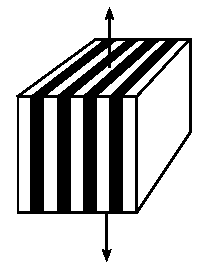
\includegraphics[width=\textwidth]{figures/voigt_mixture_rule}
            \caption{}
            \label{subfig:voigt_mixture_rule}
    \end{subfigure} \hfill
    \begin{subfigure}[b]{0.35\textwidth}
            \centering
            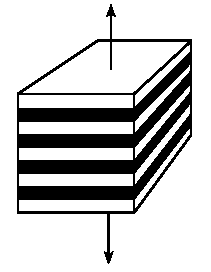
\includegraphics[width=\textwidth]{figures/reuss_mixture_rule}
            \caption{}
            \label{subfig:reuss_mixture_rule}
    \end{subfigure}
  \caption{Arrangement of the two phase in a composite yielding \subref{subfig:voigt_mixture_rule} Voigt's mixture rule and \subref{subfig:reuss_mixture_rule} Reuss' mixture rule.}
\label{fig:mixture_rules}
\end{figure}

The work of Takayanagi and coworkers \citep{takayanagiApplicationEquivalentModel1964} was, perhaps, the first to consider such an approach to model semi-crystalline polymers.
The mixture rule employed is neither the Voigt or the Reuss mixture rule, since the phases are not arranged in layers.
Instead the amorphous phase is kept at the corner of the volume element considered, with dimensions $\varphi$ and $\lambda$, as depicted in Figure~\ref{fig:model_takayanagi}.
The quantity $\varphi \lambda$ is equal to the volume fraction of amorphous polymer, supplying an extra degree of freedom that can be correlated to the distribution of one phase in the other.
A more homegeneous distribution of the amorphous phase leads to similar values for $\varphi$ and $\lambda$, while inhomogeneities in either direction favor one or the other parameter.
In \cite{takayanagiMechanicalPropertiesFine1967}, the authors consider employing similar techniques to model drawn samples of polyethylene (PE), isotactic propylene (iPP), among other crystalline polymers.
\begin{figure}[hbtp]
\centering
\begin{subfigure}[b]{0.45\textwidth}
\centering
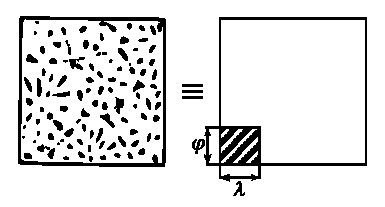
\includegraphics[width=\textwidth]{figures/takaynagi_low}
\caption{}
\label{subfig:takaynagi_low}
\end{subfigure} \hfill
	\begin{subfigure}[b]{0.45\textwidth}
		\centering
						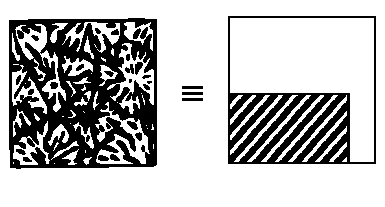
\includegraphics[width=\textwidth]{figures/takaynagi_high}
						\caption{}
						\label{subfig:takaynagi_high}
		\end{subfigure}
	\caption{Mixture model of Takayanagi et al. \citep{takayanagiApplicationEquivalentModel1964} for semi-crystalline polymers with crystallinities of \subref{subfig:takaynagi_low} about 90\% and \subref{subfig:takaynagi_high} about 50\% an their equivalent models. Black area expresses the non-crystalline region. Adapted from \cite{takayanagiApplicationEquivalentModel1964}. }
\label{fig:model_takayanagi}
\end{figure}

G'sell, Dahoun and co-workers \citep{gsellEvolutionMicrostructureSemicrystalline1994, dahounPlasticBehaviorDeformation1995} employ a mixture model using the Voigt composite model to combine the contributions from the amorphous (rubber-like) and the crystalline (viscoplastic) portions of the polymer.
They assume a temperature above the glass transition temperature and attempt to describe HDPE and PEEK subject to uniaxial traction and pure shear.
The response of the amorphous portion of the polymer is given according to the rubber elastic model in \cite{wuImprovedNetworkModels1993}, while the behavior of the crystalline phase is modeled following Parks and Ahzi \citep{parksPolycrystallinePlasticDeformation1990}.
It is based on a local-global interaction model established for polycrystalline metal \citep{molinariSelfConsistentApproach1987}, taking into account the kinematically indeterminate component of the stress in a rigid-viscoplastic crystal due the locally inextensible direction.
They consider a fully crystalline HDPE and make predictions regarding the large deformation texture developed, as well as the macroscopic stress-strain response.

% See about \cite{raoStudyStraininducedCrystallization2001}
% The model by Rao et al. \citep{raoStudyStraininducedCrystallization2001}, where the Helmholtz free energy free energy is divided according to the crystallinity, considered as an internal variable.

Ahzi et al. \citep{ahziModelingDeformationBehavior2003} model PET at large strains including strain-induced polymer crystallization at temperatures above the glass transition temperature.
The model is based on \citep{boyceConstitutiveModelFinite2000}, considering two distinct resistances, an intermolecular and network resistance.
As in the base model, the network stress is captured by the Arruda-Boyce eight-chain model (see Equation~\eqref{eq:eigth_chain_model}), and the viscous element follows the Bergström-Boyce model (see Equation~\eqref{eq:bb_reptation_model}).
The intermolecular resistance, however, is treated in a composite framework where the crystalline and amorphous phases are considered as two separate resistances coupled through either a Voigt or a Reuss like mixture rule, which yields an upper bound and lower bound for the stiffness, respectively.
The elastic elements corresponding to the crystalline and amorphous phases follow the Hencky model (see Equation~\eqref{eq:hencky_model}), and the viscous elements a model similar to the one proposed by Argon (see Equation~\eqref{eq:argon_model_free_enthalpy}), where the athermal strength $s_i$ in each phase evolves according to Equation~\eqref{eq:rate_equation_power}.

Regarding the application of the mixture rules in intermolecular resistance, there are contributions coming from the crystalline part, denoted by $c$, and the amorphous part, $a$, of the semi-crystalline polymer.
These are combined according to the degree of crystallinity, $\chi$, in two ways (see Figure~\ref{fig:ahzi_combiniations}):
\begin{itemize}
	\item in parallel, such that the gradient acting in each element is equal and the Cauchy stress is supplied by
	\begin{equation}
		\bm\sigma_A = \chi\bm\sigma_A^c + (1 -\chi)\bm\sigma_A^a.
	\end{equation}
	\item in series, such that the stress acting on both elements is the same and the plastic rate of deformation is given by
	\begin{equation}
		\mathbf D^p_A = \chi \mathbf D^{p,\ c}_A + (1 -\chi)\mathbf D^{p,\ a}_A.
	\end{equation}
\end{itemize}
\begin{figure}[hbtp]
\centering
\begin{subfigure}[b]{0.45\textwidth}
\centering
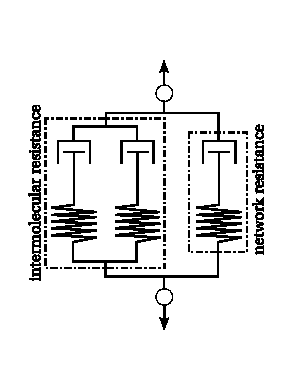
\includegraphics[width=\textwidth]{figures/ahzi_parallel}
\caption{}
\label{subfig:ahzi_parallel}
\end{subfigure} \hfill
	\begin{subfigure}[b]{0.45\textwidth}
		\centering
						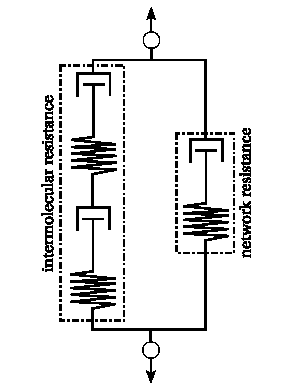
\includegraphics[width=\textwidth]{figures/ahzi_series}
						\caption{}
						\label{subfig:ahzi_series}
		\end{subfigure}
	\caption{Mixture models considered by Ahzi et al. \citep{ahziModelingDeformationBehavior2003}: \subref{subfig:ahzi_parallel} Parallel arrangement. \subref{subfig:ahzi_series} Series arrangement.}
\label{fig:ahzi_combiniations}
\end{figure}
The crystallization rate is expressed following a non-isothermal phenomenological expression based on the modified Avrami equation
\begin{equation}
  \label{eq:rate_eq_cryst}
	\dot \chi = \chi_\infty \frac{\dot\varepsilon_\text{eq}}{\dot\varepsilon_\text{ref} } m K_\text{av}(T) (-\ln(1-y))^{(m-1)/m} (1-y)\exp\left(\xi\frac{\operatorname{tr} \bm \sigma}{G_\text{comp}}\right),
\end{equation}
where $\chi_\infty$ is the maximum degree of crystallinity, $m$ is the Avrami, $\xi$ is a dimensionless model parameter, $G_\text{comp}$ is the composite bulk modulus, $\dot \varepsilon_\text{eq}$ is the applied equivalent strain rate and $\dot\varepsilon_\text{ref}$ is taken as the maximum strain rate for which experimental results are available for the calibration of the model parameters.
% See how the strain rate is defined
$K_\text{av}$ is the transformation rate function, which is defined in the case of PET as
\begin{equation}
	K_\text{av}(T) = 1.47\times 10^{-3} \left[\frac{4\pi \mathrm{Nu}}{3\chi_\infty}\right]^{1/3} \exp\left[-\left(\frac{T - 141}{47.33}\right)\right], \quad \text{(\si{\per\second}, $T$ in \si{\celsius})},
\end{equation}
with $\mathrm{Nu}$ the number density of nuclei initially present within the amorphous phase.

Strobl and co-workers \citep{hongModelTreatingTensile2004, hongModelTreatmentTensile2004, naViscousForceDominatedTensileDeformation2006} propose a somewhat similar description for polyethylene.
They also consider essentially two arms in a rheological model.
The first is a Maxwell arm with a linear spring and an Eyring dashpot in series.
The second is found through a Voigt mixture rule between a rubber elastic element and an elasto-plastic element.
These choices are supported by extensive experimental results on PEVA and PE.
% \begin{figure}
% 	\centering
% 	\includegraphics[width=.9\textwidth]{example-image-a}
% 	\caption{Model proposed by Strobl and co-workers \citep{hongModelTreatingTensile2004, hongModelTreatmentTensile2004, naViscousForceDominatedTensileDeformation2006} for semi-crystalline polymers.}
% \label{fig:strobl_model}
% \end{figure}

Makradi et al. \citep{makradiTwophaseSelfconsistentModel2005} extend this model considering a self-consistent approach based on the Eshelby result, which amounts to the use of a Maxwell arms where the properties of the elastic and viscous elements are appropriate equivalent properties as the intermolecular resistance .
The stress corresponding to the intermolecular resistance is thus given according to the Hencky model (see Equation~\eqref{eq:hencky_model}) with the isotropic elastic moduli $\bm{\mathsf D}$ is chosen following the self-consistent method proposed by Hill \citep{hillSelfconsistentMechanicsComposite1965}.
The flow rule for the viscous element is given by Equation~\eqref{eq:flow_rule_directions}, neglecting the volumetric part.
The strain rate, $\dot \gamma_\text{dev}$ is defined as an average strain rate, $\dot{\bar\gamma}$, according to
\begin{equation}
	\label{eq:def_avg_strain_rate}
	\dot{\bar\gamma} = \frac{1}{V}\int_V \dot \gamma\ dV = \frac{1}{V}\sum_i V_i \dot{\gamma}_i,
\end{equation}
where
\begin{equation}
	\dot \gamma_i = \frac{1}{V_i}\int_{V_i} \dot \gamma\ dV_i,
\end{equation}
with $V_i$ the volume of the $i$th phase and $V$ representing the total volume.
For each phase, the flow rule is also given by Equation~\eqref{eq:flow_rule_directions}, neglecting the volumetric part, with the strain rate in each phase following a power law (see Equation~\eqref{eq:flow_rule_power_law}).
Thus, the average strain rate is also described by a power law, with an average strength $\bar s$.
It can be shown, taking into account Eshelby's results for an ellipsoidal inclusion, that
\begin{equation}
	\frac{\dot \gamma_i}{\dot{\bar \gamma}} = \frac{5}{3} - \frac{2}{3}\frac{s_i}{\bar s} \left(\frac{\dot \gamma_i}{\dot{\bar \gamma}}\right)^{1/n},
\end{equation}
which combined with Equation~\eqref{eq:def_avg_strain_rate} and the corresponding power law, yields the average strain rate.
The authors employ the same description for the evolution of the crystallinity as \cite{ahziModelingDeformationBehavior2003}, in addition to the Flory’s theory to predict the onset of crystallization as a function of the processing temperature and the extension of the polymer molecules.
Later Regrain et al. \citep{regrainMultimechanismModelsSemicrystalline2009} extend the DID models to semi-crystalline models also employing a self-consistent scheme to consider the contribution of both phases.

Dusunceli and Colak \citep{dusunceliModellingEffectsDegree2008} extend the viscoplasticity theory based on overstress (VBO) to include crystallinity.
This is achieved describing both phases employing the VBO model and considering their contributions using either a Voigt or a Reuss mixture rule.
The authors validate their model using polyethylenes (UHWPE and XLPE) as well as PTFE.

Ayoub et al. \citep{ayoubModellingLargeDeformation2010, ayoubEffectsCrystalContent2011} present a model very similar to \cite{ahziModelingDeformationBehavior2003} and \cite{boyceConstitutiveModelFinite2000} to describe the mechanical behavior of HDPE.
The inelastic mechanisms involve two parallel elements: a visco-hyperelastic network resistance acting in parallel with a viscoelastic–viscoplastic intermolecular resistance where the amorphous and crystalline phases are explicitly taken into consideration.
The semi-crystalline polymer is considered as a two-phase composite in a way similar to what has already been described.
In the first contribution, both the crystalline and amorphous resistances are modeled employing the VBO model.
Their contributions to the intermolecular resistance are incorporated through a Voigt mixture rule (see Equation~\eqref{eq:voigt_mixture_rule}).
In the second contribution, the elastic and viscous elements in crystalline and amorphous resistances are modeled employing Hencky's model (see Eqaution~\eqref{eq:hencky_model}) and a simplified version of Argon's model (see Equation~\eqref{eq:argon_model_free_enthalpy}).
They employ a modified Voigt mixture rule, where the contribution to the intermolecular resistance to the coming from the crystalline and amorhpous phases are combined through
\begin{equation}
  \label{eq:mod_voigt_mixture_rule}
  \bm \sigma = \chi^\beta \bm \sigma_c + (1-\chi)^\beta \bm \sigma_a,
\end{equation}
where $\beta$ is an appropriate exponent.
It is found from a fit of the Young modulus as a function of the degree of crystallinity, as shown in Figure~\ref{fig:deg_cryst_stiff}.
Comparing with experimental results obtained for polyethylene samples containing degrees of crystallinity between 15 and 72\%, the model is able to accurately capture the change in response with crystallinity before the strain hardening becomes evident.
Different material parameters for each crystallinity are needed to capture the strain hardening at large strains (> 1).
A similar model can be found in \cite{abdul-hameedTwophaseHyperelasticviscoplasticConstitutive2014}, where the major difference is the substitution of the Maxwell arm in the network resistance for two arms, one corresponding to the amorhpous contribution and other to the crystalline contribution.
They are combined as shown in Equation~\eqref{eq:mod_voigt_mixture_rule}.
This approach allows for a better fit across different degrees of crystallinity when strain hardening becomes evident employing the same material parameters.
Very recently, Cundiff et al. \citep{cundiffModelingViscoplasticBehavior2022} propose another model where the inclusion of the crystallinity is achieved through the modified Voigt mixture rule (see Equation~\eqref{eq:mod_voigt_mixture_rule}).
Regarding the constitutive description of each phase it employs much of the same laws found in \cite{ahziModelingDeformationBehavior2003} and \cite{chowdhuryEffectsManufacturingInducedVoids2008}, already described.
It describes strain rate crystallization through a rate equation similar to Equation~\eqref{eq:rate_eq_cryst}.

Lastly, the two-phase model of Cangemi and Meimon for semi-crystalline polymers \citep{cangemiTwoPhaseModelMechanical2001} achieves the inclusion of the bulk crystallinity into the description of a semi-crystalline polymer in a different way.
It is based on the continuum mixture theory such that according to the microstructure of semi-crystalline polymers, the free amorphous phase is assumed comparable to a fluid which saturates the complementary space to that of the solid structure, the crystalline phase plus the rigid amorphous phase.

\section{Micromechanical models}

In addition to bulk crystallinity, the final set of models includes some geometric considerations at the micro scale.
Accordingly, a micromechanical modeling based on the laminar composite approach was proposed by Lee et al. \citep{leeMicromechanicalModelingLarge1993, leeSimulationLargeStrain1993}.
In this model, a rigid-viscoplastic amorphous phase using 8-chain model (see Equation~\eqref{eq:eigth_chain_model}) was added, and Sachs/Taylor hybrid interaction law was used to relate the mechanical properties of microscopic two-phase inclusion and an aggregation of the inclusions.
In these models, a crystalline polymer is regarded as a polycrystalline aggregate of randomly distributed crystallites which plastically deform in a co-operative manner.
It does not consider the mesoscopic structure of the polymer.

According to Uchida et al. \citep{uchidaMicroMesoMacroscopic2013}, these models were then improved to more realistic elasto-viscoplastic models by Nikolov et al. \citep{nikolovMicroMacroConstitutive2000, nikolovMultiscaleConstitutiveModeling2002} and van Dommelene et al. \citep{vandommelenMicromechanicalModelingElastoviscoplastic2003}
In a similar vein, Guan et al. \citep{guanMicromechanicalModelElastic2004} present a micromechanical analysis of the elastic properties of semicrystalline thermoplastic materials.

Bedoui et al. \citep{bedouiMicromechanicalModelingIsotropic2006} considers a micromechanical model applied to infinitesimal strain, concluding that the spherulitic mesostructure does not affect the response of the material at that level of strain.
The phase of the amorphous part of the semi-crystalline polymers has a noticeable impact on the stiffness of the polymer.
There is a moderate agreement between the predictions and the experimental results.

Alternatively, Uchida and coworkers \citep{uchidaMicroMesoMacroscopic2013} developed a large deformation finite element homogenization model of spherulitic HDPE.
This in contrast to the previously described models, because the interaction laws applied in these models have no geometric information, compatibility and equilibrium in the spherulite cannot be taken into consideration.
Since Uchida's and coworkers model directly solves both the microscopic and mesoscopic displacement fields using FE-based homogenization scheme, compatibility and equilibrium between adjacent microstructure in the spherulite are automatically satisfied.
According to the authors, when macroscopic response and texture evolution are required, the former micromechanical-based model are suitable.
Meanwhile, homogenization-based model is proper when distributions of strain and stress in the spherulite are required.
Regarding the size of the representative domain, Teixeira-Pinto et al. \citep{teixeira-pintoSizeEstimationRepresentative2016} claim that it significantly exceeds the size of a single spherulite.


% \colorbox{BrickRed}{Consider saying something about deformation maps \cite{frostDeformationmechanismMapsPlasticity1982}, \cite{odonnellComputerProgramGenerating1991} \cite{kawasakiManyFacetsDeformation2013, vanloockDeformationFailureMaps2018, richardPredictingPlasticityDisordered2020}}
